\chapter{Úvod}

Tato bakalářská  práce je rozdělena do šesti kapitol.

\begin{enumerate}
  \item \textbf{Úvod} - Úvodní kapitola.
  \item \textbf{Radioamatéři} - V druhé kapitole (\ref{radioamateri}) je popsána historie amatérského rádia
(\ref{radioamateri_hist}) a také jeho aktuální stav dnes (\ref{radioamateri_dnes}).
  \item \textbf{Rozbor zadání} - V třetí kapitole ...
  \item \textbf{Návrh aplikace} - Čtvrtá kapitolá (\ref{navrh}) stručně popisuje návrh 
komunikačního protokolu (\ref{navrh_protokol}), serverové aplikace (\ref{navrh_server}), klientské knihovny 
(\ref{navrh_knihovna}) a samotné klientské aplikace (\ref{navrh_klient}).
  \item \textbf{Implementace} - V páté kapitole (\ref{implementace}) je popsána implementace všech součástí
zmíněných v kapitole čtvrté (\ref{navrh}). V podkapitole o implementaci serverové aplikace (\ref{implementace_server})
je popsána implementace databázového rozhraní (\ref{implementace_db}), modulů (\ref{implementace_moduly}),
seznam implementovaných modulů (\ref{implementace_moduly_list}) a logování (\ref{implementace_logovani}). Dále je
zde popsána implementace klientské knihovny (\ref{implementace_knihovna}) a samotného klienta (\ref{implementace_klient}).
  \item \textbf{Závěr} - V šesté kapitole (\ref{zaver}) ...
\end{enumerate}

\chapter{Radioamatéři}
\label{radioamateri}

V této kapitole je stručně popsána historie amatérského rádia a jsou zde vysvětleny důležité pojmy používané dále v práci.
Podkapitola \ref{radioamateri_hist} a \ref{radioamateri_dnes} byla převzata z \cite{crk_hist}.

\section{Historie amatérského rádia}
\label{radioamateri_hist}
Prvotní motivací pro vznik amatérského rádia byla myšlenka našich předků rádio nejen poslouchat, ale také vysílat.
To dalo vzniknout novému druhu zábavy - amatérskému vysílání (HAM Radio). Lidem, kteří vysílali se pak začalo říkat 
radioamatéři.

Amatérské rádio se začalo rychle šířit po první světové válce hlavně díky vlivu rozhlasu. V těchto dobách radioamatéři značně
přispěli k získání znalostí o využití celého spektra radiových vln. Vysílali na dlouhých a středních vlnách, které byly do té doby
považovány za bezcenné, a také na vlnách krátkých, o jejichž existenci se nevědělo vůbec.

První pokusy o transatlantické spojení začaly lákat také Pravoslava Motyčku - prvního známého radioamatéra u nás.
Koncem roku 1924 navázal Motyčka první spojení v Československu. 
Díky Motyčkově inspiraci bylo u nás kolem 30. let 20. století až několik set radioamatérů.

Dalším významýn rokem byl rok 1928, kdy byl ruský radioamatér prvním, kdo zachytil volání vzducholodi ITALIA,
která ztroskotala na cestě od severního pólu. To změnilo pohled na amatérské rádio, do té doby vnímané spíše jako zábava než
příliš užitečná věc. Při mnoha pohromách na celém světě často pomohla připravenost radioamatérů poskytnout rychlé spojení do
jiných míst.

\section{Amatérské rádio dnes}
\label{radioamateri_dnes}

Základním pilířem amatérského rádia je vysílání na krátkých vlnách umožňují spojení do celého světa včetně exotických zemí.
Řada radioamatérů se snaží a spojení s co nejvíce exotickými zeměmi. Této zálibě říkáma DX provoz.
Po úspěšně navázaném spojení si radioamatéři vyměnují QSL lístky (potvrzení o navázaném spojení formátu pohlednice). Cílem je
získání QSL lístků z co mozná nejvíce zemí světa (ideálně všech).

Pro kvalitní příjem profesionálního vysílání (například FM rozhlas nebo televize) je potřeba být od výsilače vzdálen maximálně
v desitkách kilometrů. Radioamatéři se při svých vysíláních snaží tyto limity překonat a provádět spojení na co největší
vzdálenosti. K tomu využívají kromě techniky také dobrých znalostí faktorů, které ovliňují šíření krátkých vln. Těmi jsou například
rozhraní teplých a studených mas vzduchu nebo polární záře. Profesionálové se nemohou na tyto přechodné faktory spolehnout, ale 
radioamatéři jsou díky nim schopni navázat spojení až na tisíce kilometrů

Na řadě vysokých budov a kopců pracují pozemní radioamatérské převaděče. Převaděč přeposílá signál přijatý na na jedné frekvenci
na frekvenci jinou. Radioamatéři se tak mohou pomocí převaděče dovolat na velké vzdálenosti i s použitím vysílačů o malém výkonu
(často jde o kapesní radiostanice)

V počátcích 60. let byla také vypoštěna první radioamatérská družice. Dnes jich existuje několik desítek.
Družice pokrývají, podobně jako běžné televizní satelity, kruh o průměru zhruba 4000 km. 
Narozdíl od geostacionárních televizních satelitů však amatérské družice kolem Země obíhají.
Díky tomu jsou schopny pokrýt postupně signálem všechny obydlené oblasti.

V radioamatérském vysílání se rovněž konají závody. Cílem je například v určitém čase navázat spojení s co nejvíce jinými
amatérskými stanicemi v co nejvíce zemích. Jinou variantou je například součet vzdáleností všech spojení vykonaných za určitý
čas.

Morseova abeceda byla prvním dorozumívacím prostředkem používaným v amatérském rádiu a je radioamatéry používána dodnes.
Hlavním přínosem morseovy abecedy je její velká odolnost proti rušení, diký níž lze překonat velké vzdálenosti i s malým
výkonem. Další výhodou je to, že odbourává jazykové bariéry, protože se komunikuje převážně pomocí zkratek. Při hlasové komunikaci
je mezinárodním jazykem angličtina a využívá se amplitudové modulace SSB nebo FM modulace.

Nejnovějším systémem pro zakódování řeči je je packet 
radio. V podstatě se jedná o radioamatérský Internet, kde se informace přenáší pomocí modifikace protokolu X.25. 
Síť packet radia pokrývá celý vyspělý svět, její součástí jsou i BBS (databanky pro ukládání a výměnu informací) a
elektronická pošta. Poslat e-mail kamarádovi do Austrálie nemusíte jen po Internetu,
ale také amatérským packet radiem, a nemáte-li nic lepšího na práci, můžete trávit hodiny zkoumáním nových zpráv i
zajímavých programů v desítkách BBS po celé Evropě.

Samozřejmě jde vysílat i obrazové signály. Dlouhou tradici má tzv. pomalá televise (SSTV),
jaká byla použita i u přenosu obrazu z prvních přistání amerických astronautů na Měsíci,
dnes se experimentuje s různými digitálními přenosy a na UHF kmitočtech je možné použít i klasickou televisní normu.

Z ryze sportovních aktivit je dobře známý rádiový
orientační běh. Cílem je v nejkratším čase najít pomocí
přijímače v terénu ukryté zamaskované vysílače. 
Tyto sporty jsou atraktivní a pěstují je i lidé, kteří se jinak o radioamatérství příliš nezajímají.

\section{Důležité pojmy}
\label{radioamateri_pojmy}

V této podkapitole jsou popsány důležité pojmy používané mezi radioamatéry, které jsou také použity dále v této práci.

\subsection{Volací značka}

Každá stanice má přidělenu jedinečnou volací značku, kterou operátor stanice uvádí při každém spojení.
První dva znaky značky jsou určeny podle přehledu mezinárodních volacích znaků přidělených dané zemi.
Dalším znakem je číslo 0-9. Kombinaci těchto tří znaků se říká prefix. Zbytek značky je tvořen jedním až čtyřmi znaky.

Na základě prefixu tak lze určit zemi, ze které daný operátor pochází a tak i jeho přibližnou polohu. K tomu slouží seznam DXCC
obsahující všechny aktuálně používané prefixy a informace k nim.

\subsection{ITU zóny}

Jedním z možných rozdělení světa na menší celky je jeho rozdělení do takzvaných ITU zón.
Systém je pojmenován podle organizace International Telecommunications Union. Svět je rozdělen do celkem 
89 zón ve třech regionech.

\begin{figure}[h]
\centering
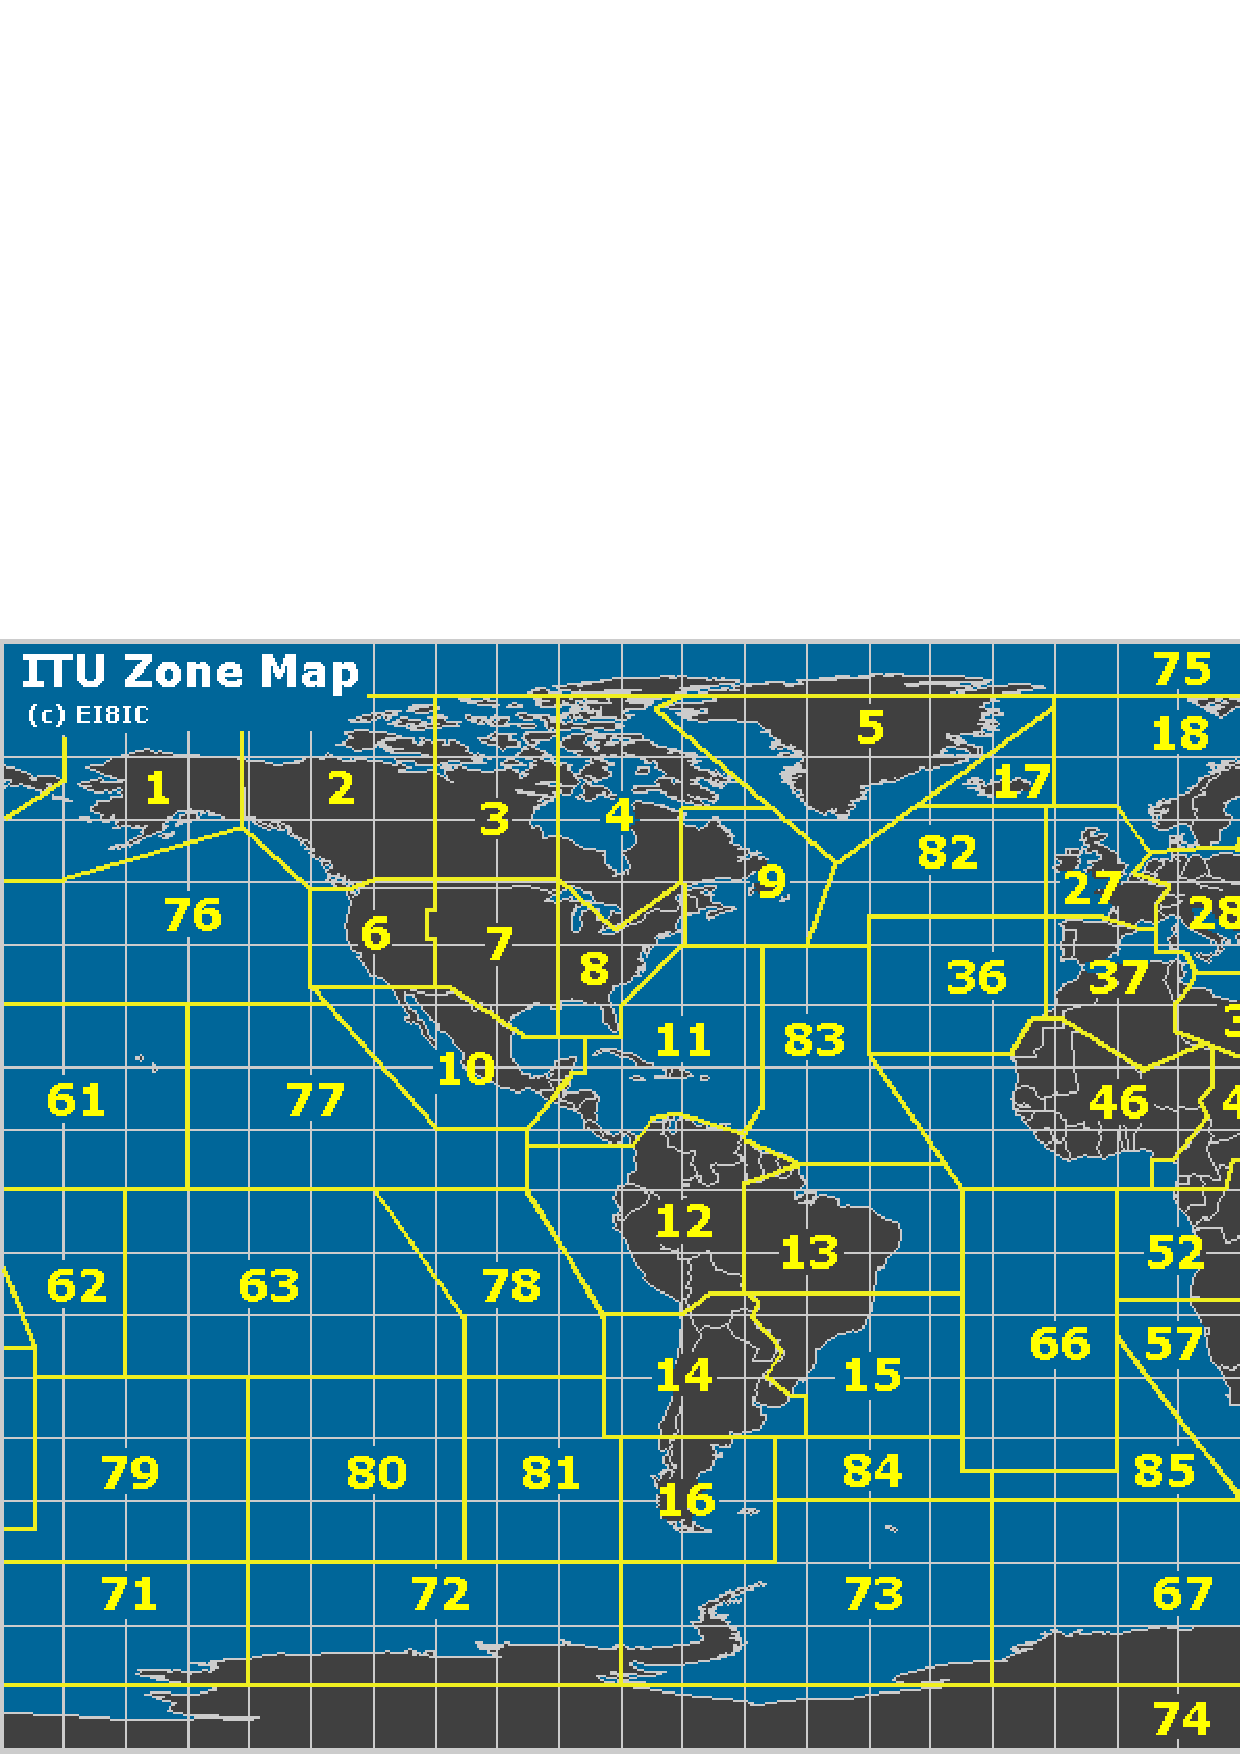
\includegraphics[trim=0cm 0cm 0cm 0cm, scale=0.4]{fig/itu-zone}
\caption{Rozdělení ITU zón.}
\label{fig:FigureExample}
\end{figure}

\subsection{CQ zóny}

Dalším z možných rozdělení světa používaných radioamatéry je dělení na CQ zóny, pojmenované podle časopisu CQ.
Jde o pouze 40 zón.

\begin{figure}[h]
\centering
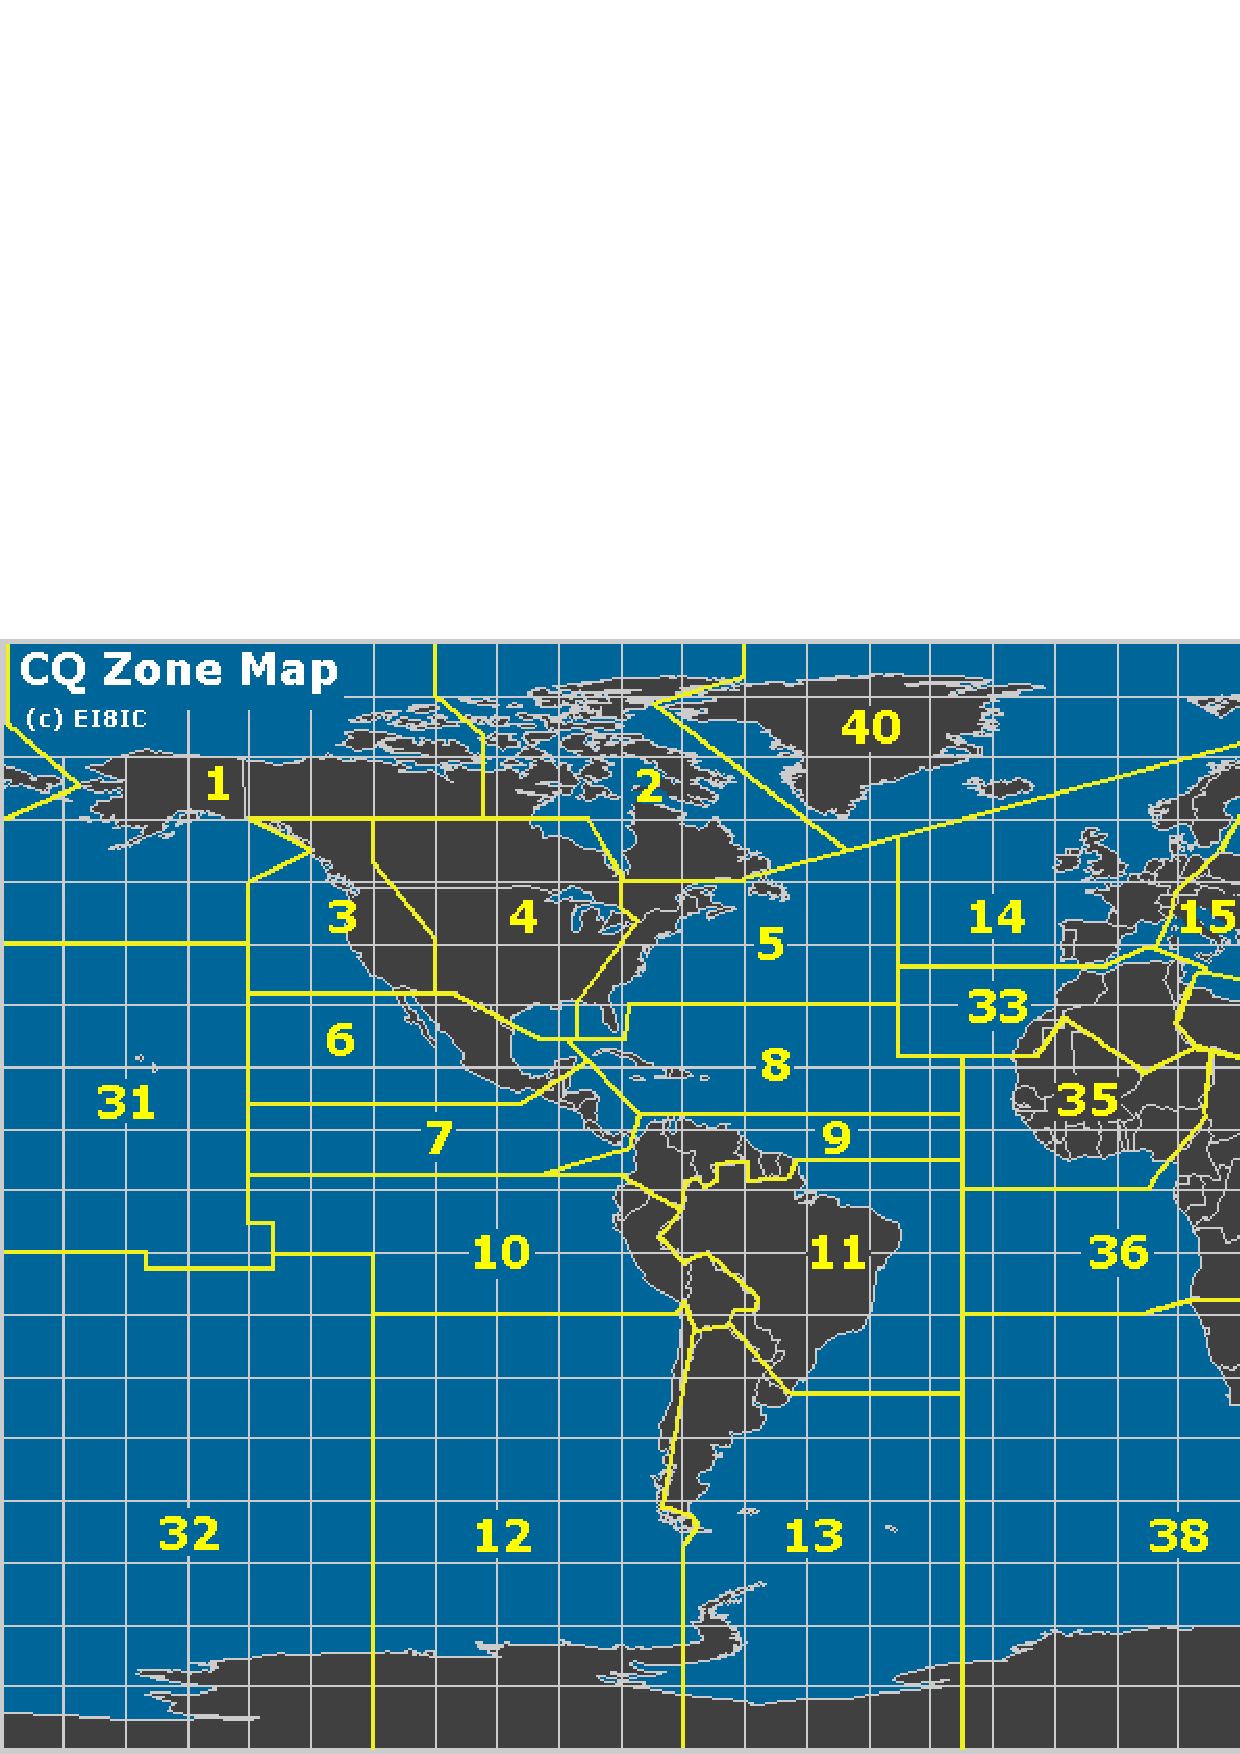
\includegraphics[trim=0cm 0cm 0cm 0cm, scale=0.4]{fig/cq-zone}
\caption{Rozdělení CQ zón.}
\label{fig:FigureExample}
\end{figure}

\subsection{QTH lokátor}

Poslední z používaných systémů pro rozdělení světa je QTH lokátor. Jde o rozdělení na základě zeměpisné šířky a délky.
Země je rozdělena do obdélníků o velikosti 1\degree x 2\degree.

\begin{figure}[h]
\centering
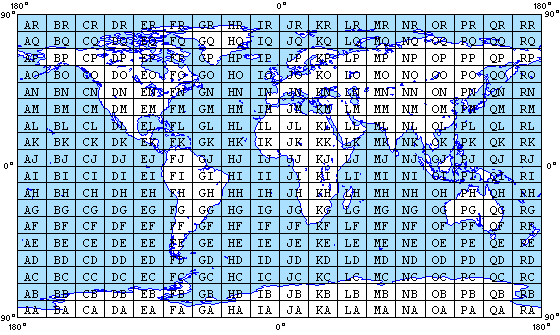
\includegraphics[trim=0cm 0cm 0cm 0cm, scale=0.7]{fig/QTH_locator}
\caption{Mapa rozdělení pomocí QTH lokátoru.}
\label{fig:FigureExample}
\end{figure}

\subsection{QTH lokátor}

\section{Služby používané radioamatéry}
\label{radioamateri_sluzby}

Díky rozšiřování Internetu se začaly rozvíjet i služby provozované radioamatéry pro další radioamatéry. V této podkapitole
jsou stručně popsány služby, kterých je v aplikaci využito a se kterými aplikace umí spolupracovat.

\subsection{DXCluster}

DXCluster je komunitní službou umožňující radioamatérovi informovat ostatní radioamatéry o tom, kdo aktuálně vysílá. Kromě
volací značky se posílá i poloha a frekvence, na které radioamatér vysílá. Díky této službě tak lze jednodušeji navazovat
spojení. Protokol služby DXCluster je postaven na službě telnet a není nikterak složitý. Lze jej jednoduše číst a zpracovávat.

\subsection{QRZ.com}

QRZ.com je největší databází radioamatérů z celého světa. Na základě volací značky lze s její pomocí zjistit různé detailní
informace (například jméno nebo přesnou polohu) o jejím majiteli. Vyhledávat lze i pomocí speciálního webového rozhraní
postaveného na technologii XML. To je velmi výhodné pro tvorbu aplikací využívajících QRZ.com pro zjištění informací o
operátorech. XML rozhraní umožňuje přihlásit se ke službě QRZ.com a provést vyhledání na základě volací značky.

\chapter{Současné logovací aplikace}
\label{soucasnost}

V této kapitole jsou posány aplikace používané současnými radioamatéry pro logování spojení. Každá aplikace je stručně
popsána a jsou zmíněny i její klady a zápory. Na základě této kapitoly bude vytvořen základní návrh aplikace.

\section{Logger32}

Logger32 je jednou z nejznámějších logovacích aplikací pro operační systém Windows. Jeho hlavní výhodou je přehledné a funkční
uživatelské rozhraní rozhraní a podpora přídavných pluginů.

\begin{figure}[h]
\centering
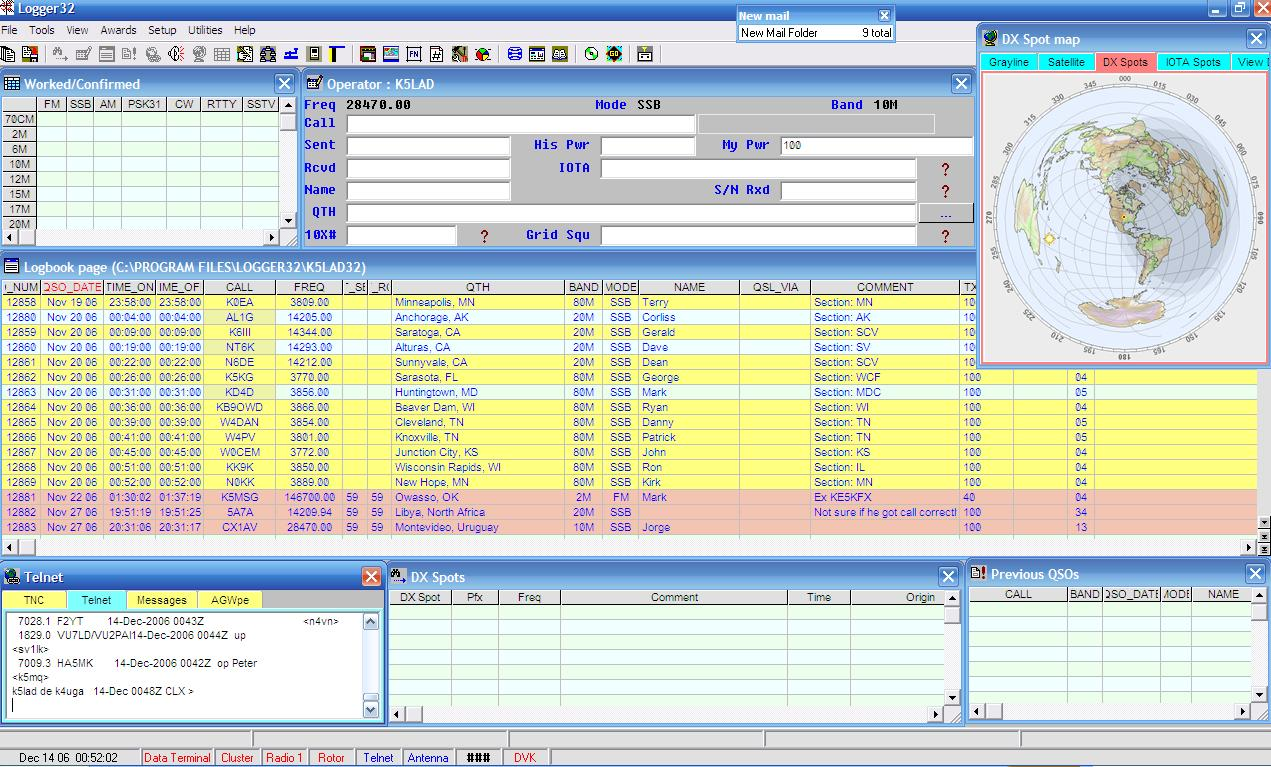
\includegraphics[trim=0cm 0cm 0cm 0cm, scale=0.33]{fig/logger32}
\caption{Uživatelské rozhraní Logger32.}
\label{fig:FigureExample}
\end{figure}

Lze vytvářet pluginy pro vyhledávání detailních informací na základě volací značky a také pluginy vytvářející externí okno
s informacemi rozšiřující informace. Logger32 také umožňuje ovládání radiostanice.

Hlavní nevýhodou aplikace Logger32 je její závislost na systému Windows. Moderním trendem dnešní doby je programování multiplatformních
aplikací. Další nevýhodou je absence zdrojových kódů, takže je rozšířitelnost aplikace limitována rozhraním modulů definovaným
tvůrcem aplikace.
Mezi nevýhody můžeme řadit také nemožnost použití externí databáze jako je například SQLite3 nebo MySQL. Problémem může rovněž být
situace, kdy chce uživatel zalogovat nové spojení z mobilního telefonu nebo jiného zařízení s nestandardním operačním systémem. V
dnešní době je důležitým faktorem při tvorbě aplikací důraz na jejich použitelnost na širokém počtu zařízení.

\section{CQRLOG}

CQRLOG je nejpoužívanějším logovacím nástrojem z řad multiplatformních aplikací. Je možné jej používat jak v systému
Windows, tak v Linuxových distribucích.

\begin{figure}[h]
\centering
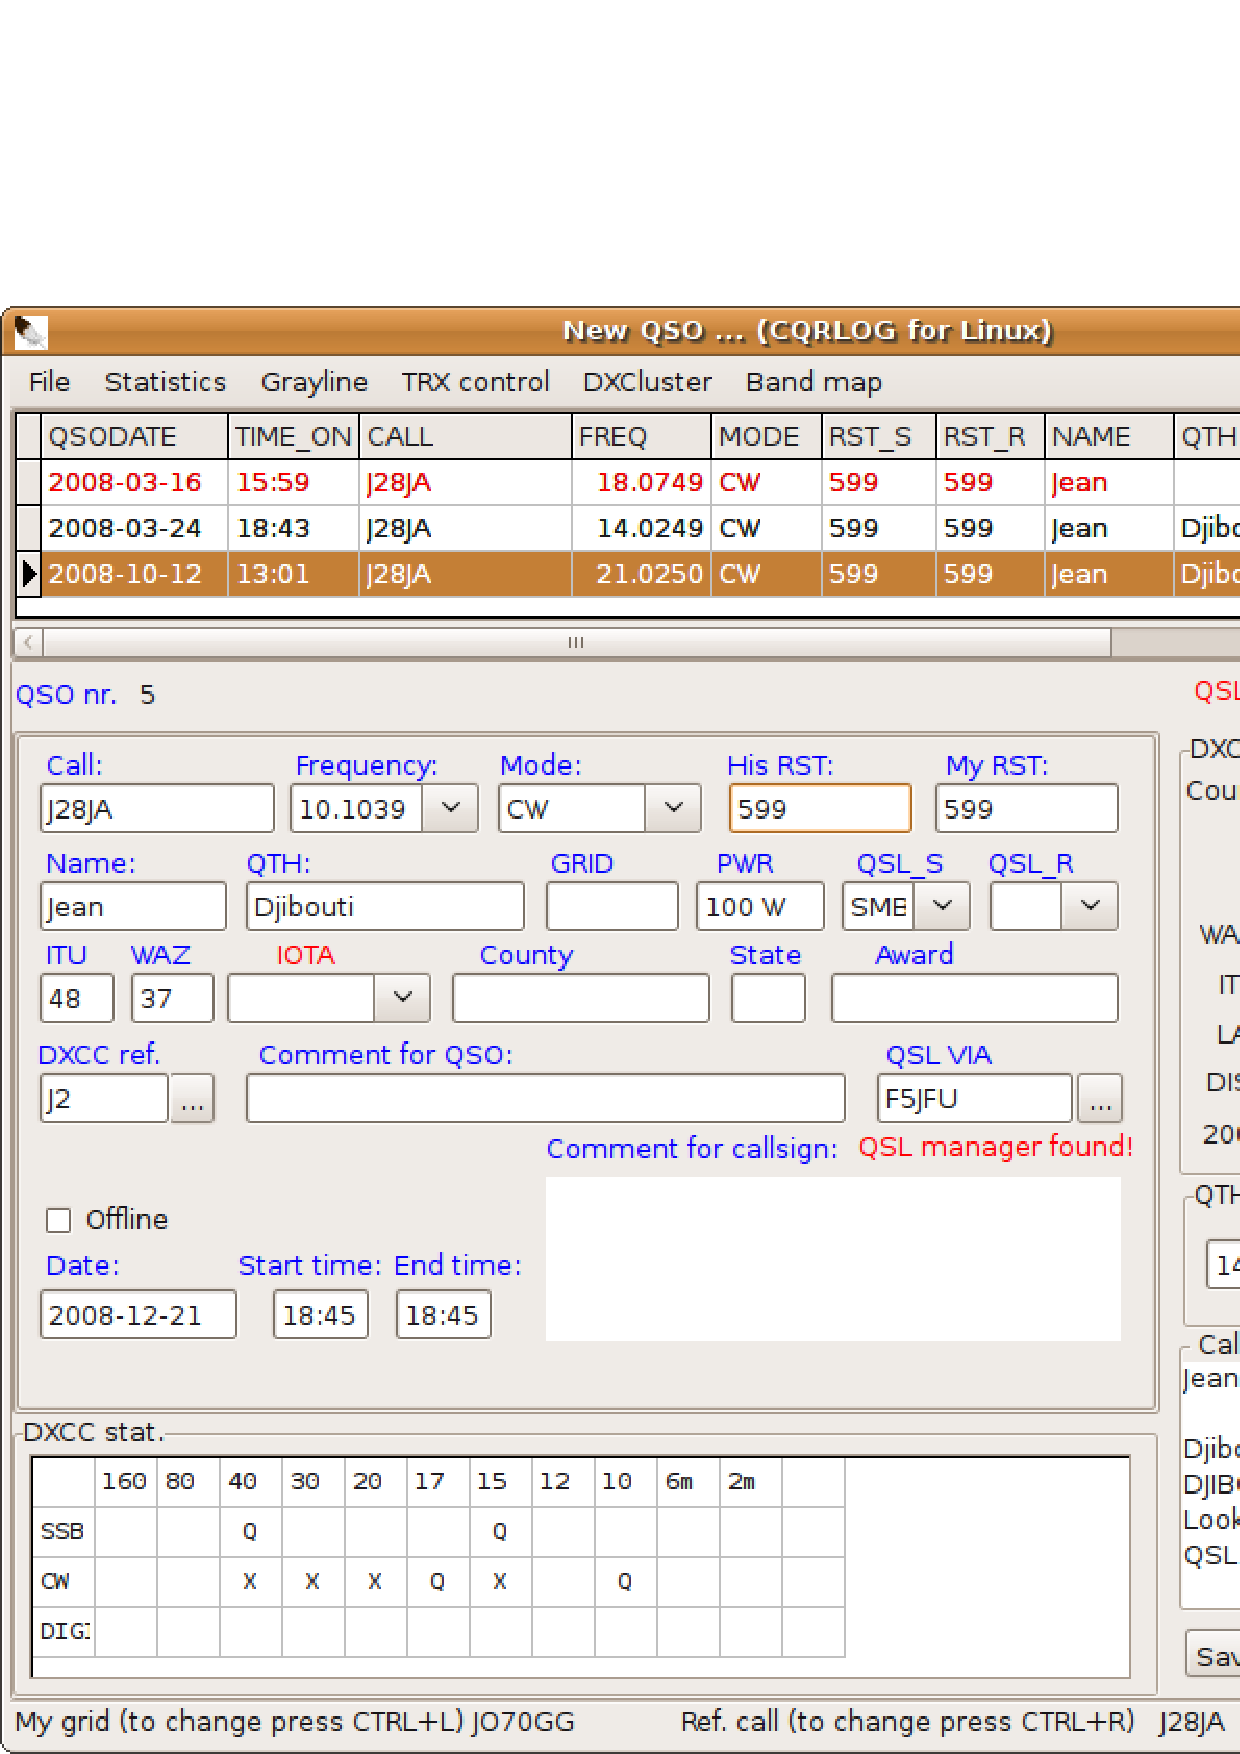
\includegraphics[trim=0cm 0cm 0cm 0cm, scale=0.5]{fig/cqrlog}
\caption{Uživatelské rozhraní CQRLOG.}
\label{fig:FigureExample}
\end{figure}

Jeho uživatelské rozhraní je jednodušší než rozhraní programu Logger32 a je také více přehledné. Na druhou stranu však
chybí podpora rozšíření formou pluginů. K dispozici jsou zdrojové kódy v jazyce Delphi. Volba tohoto programovacího jazyka
značně ztěžuje (až znemožňuje) tvorbu oficiálních instalačních baličků pro linuxové distribuce.

CQRLOG umožňuje použítí
MySQL databáze, ale návrh aplikace znemožňuje jednoduchou změnu databázové aplikace. Také volba MySQL databáze pro použití 
v desktopové aplikaci může být vnímána jako negativum. Návrh CQRLOGu rovněž nedefinuje rozhraní pro jednoduché přidávání nebo úpravu
záznamů pomocí aplikací třetích stran a není tak jednoduché postavit další aplikaci nad CQRLOGem.

\section{HAM Radio Deluxe}

\begin{figure}[h]
\centering
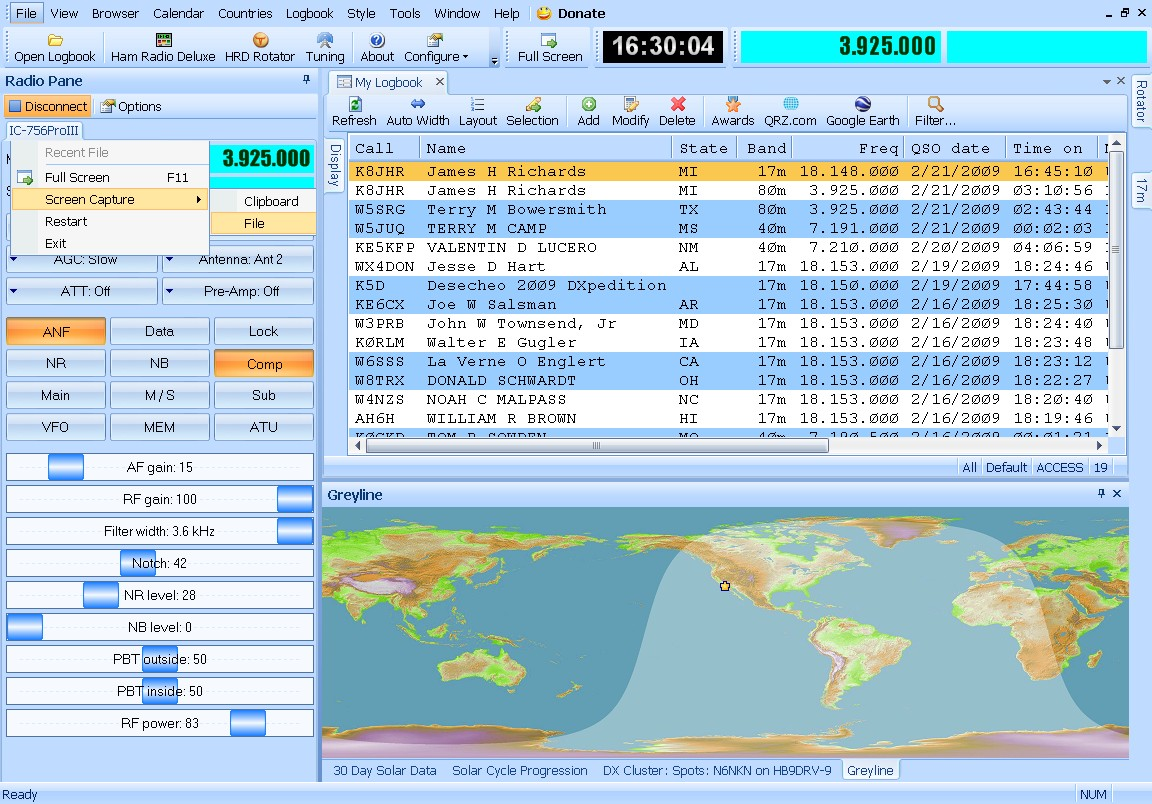
\includegraphics[trim=0cm 0cm 0cm 0cm, scale=0.33]{fig/hrd}
\caption{Uživatelské rozhraní HAM Radio Deluxe.}
\label{fig:FigureExample}
\end{figure}

\chapter{Návrh aplikace}
\label{navrh}

Cílem této kapitoly je popsání návrhu aplikace a použitého komunikačního protokolu.

Na základě rozboru současně používaných aplikací z předchozí kapitoly vyplynuly základní požadavky
na výslednou aplikaci.

\begin{itemize}
\item \textbf{Multiplatformnost} - Návrh aplikace musí počítat s možností jejího spouštění na různých operačních systémech
a platformách.
\item \textbf{Klient-server architektura} - Jádro programu je tvořeno serverem.
Server umožňuje vedení deníků více uživatelů zároveň a poskytuje rozhraní pro přídavné moduly.
Klientská aplikace se připojí k serveru a prostředníctvím komunikačního protokolu s ním komunikuje.
Díky tomuto rozdělení je možné přidávat záznamy do centrální databáze z více zařízení a pracovat
tak všude se stejnými daty. Využití klient-server architektury je výhodné také pro soutěže, kdy může vyhodnocení
výsledků všech účastníků proběhnout současně na centrálním místě.
\item \textbf{Modulárnost} - Serverová aplikace je založena na modulech. Moduly jsou speciální knihovny rozšiřující funkce
serveru. Moduly umí zpracovávat klientské požadavky a je jim umožněn přístup k deníkům jednotlivých uživatelů. Díky použití modulů
je zajištěna jednoduchá rozšíritelnost aplikace o nové funkce bez nutnosti změny jejího jádra.
\item \textbf{Uložení dat} - Záznamy jednotlivých uživatelů jsou uloženy v databázi SQLite3. Návrh aplikace
však počítá s možností použití různých formátů pro uložení uživatelských dat.
\item \textbf{Oddělení grafického rozhraní od komunikace se serverem} - Klientská aplikace využívající grafického rozhraní
je oddělena od nízkoúrovňové komunikace se serverem díky klientské knihovně. Klientská knihovna obsahuje základní funkce
pro komunikaci se serverem a umožňuje použití libovolného grafického rozhraní bez zbytečné duplikace kódu.
\end{itemize}

Aplikace se tedy skládá z modulárního serveru, klientské knihovny a grafického uživatelského rozhraní.
V následujících podkapitolách jsou jednotlivé části stručně popsány.

\begin{figure}[h]
\centering
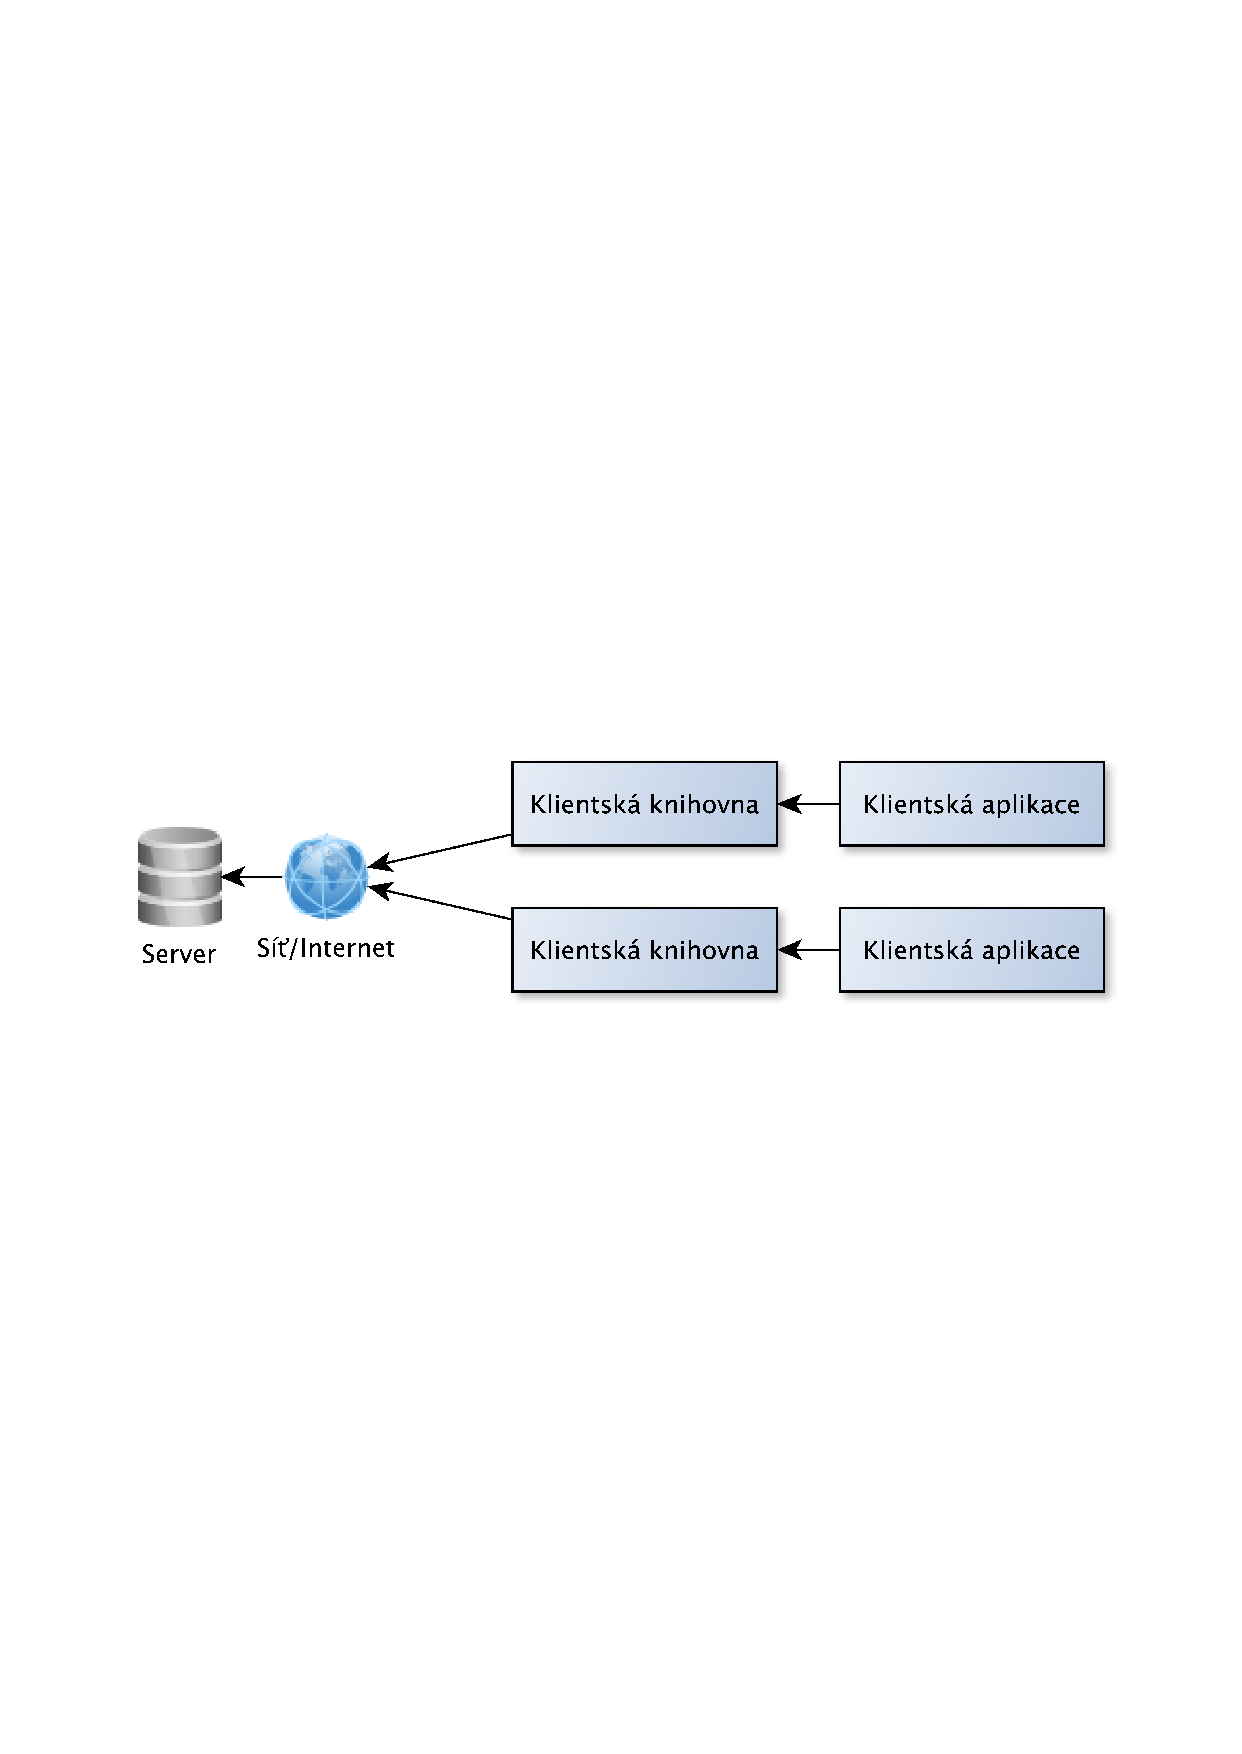
\includegraphics[trim=12cm 12cm 12cm 12cm, scale=0.8]{fig/princip}
\caption{Základní činnost programu.}
\label{fig:FigureExample}
\end{figure}

\newpage
\section{Návrh komunikačního protokolu}
\label{navrh_protokol}

Byl zvolen protokol inspirovaný protokolem HTTP \cite{http}, převážně kvůli jeho jednoduchosti a účelnosti z hlediska modularity.
Jednotlivé moduly serveru mají své vlastní URI a klientské požadavky jsou pak směrovány podle URI na konkrétní modul,
který vygeneruje odpověď poslanou klientovi.

Protokol je zpětně kompatibilní s protokolem HTTP, ale jsou použity jen některé jeho části. Komunikace probíhá v režimu
požadavek-odpověď.

Data přenášená protokolem HTTP jsou ve formátu CSV \cite{csv}, kde první řádek reprezentuje hlavičku dat. Standardní názvy
sloupců ve hlavičce protokolu jsou:
\begin{itemize}
\item \textbf{id} - ID záznamu v logu. Koresponduje s ID v databázi a slouží jako klíč pro vybrání konkrétního řádku.
\item \textbf{user\_id} - ID uživatele, jemuž záznam v logu patří.
\item \textbf{qsodate} - Datum záznamu ve formátu unixového timestampu.
\item \textbf{callsign} - Volací značka (například OK2JRQ).
\item \textbf{mode} - Mód spojení.
\item \textbf{qth} - QTH lokátor (Maidenhead Locator).
\item \textbf{name} - Jméno operátora.
\item \textbf{latitude} - Zeměpisná šířka.
\item \textbf{longitude} - Zeměpisná délka.
\item \textbf{conty} - Okres.
\item \textbf{continent} - Zkratka kontinentu.
\item \textbf{cq} - CQ zóna.
\item \textbf{itu} - ITU zóna.
\end{itemize}

Jednotlivé moduly serveru však mohou použít i své vlastní názvy sloupců pro položky, které nejsou v tomto seznamu.

\subsection{Ukázky použití protokolu}

\subsubsection{Vyžádání logu}

Tento příklad ukazuje použití protokolu pro získání všech záznamů z logu.

Dotaz na modul poskytující URI "/logbook":
\begin{verbatim}
GET /logbook HTTP/1.1


\end{verbatim}
Odpověď serveru:
\begin{verbatim}
HTTP/1.1 200 OK
Content-Type: text/hamlog
Content-Length: 74

id;user_id;callsign;date;qth;loc
1;1;TEST;2011;qt;
2;1;LKS;2011;;location
\end{verbatim}

\subsubsection{Editace záznamu}

TODO

Dotaz na modul poskytující URI "/logbook":
\begin{verbatim}
GET /logbook HTTP/1.1


\end{verbatim}
Odpověď serveru:
\begin{verbatim}
HTTP/1.1 200 OK
Content-Type: text/hamlog
Content-Length: 74

id;user_id;callsign;date;qth;loc
1;1;TEST;2011;qt;
2;1;LKS;2011;;location
\end{verbatim}

\subsection{Přihlášení uživatele}

Přihlášení je prováděno metodou Digest Access Authentication definovanou v RFC 2617 \cite{rfc2617}. Díky tomu se heslo neposílá
při přihlášení po síti a je možné jej na straně serveru ukládat zahashované. Nehrozí tak jeho možný odposlech během přihlášení.

\subsubsection{Ukázka přihlášení uživatele}

Dotaz na modul poskytující URI "/login":
\begin{verbatim}
GET /login HTTP/1.1

\end{verbatim}

Odpověď serveru vybízí uživatele k přihlášení podle RFC 2617 \cite{rfc2617}:
\begin{verbatim}
HTTP/1.0 401 Unauthorized
Content-Type: text/html
Content-Length: 14
WWW-Authenticate: Digest realm="realm@hamlog",qop="auth,auth-int",nonce="dcd98b7102dd2f0e8b11d0f600bfb0c093",opaque="5ccc069c403ebaf9f0171e9517f40e41"

Authentication
\end{verbatim}

Klient se přihlásí s použitím správného jména a hesla, které je všask přenášena zahashované:
\begin{verbatim}
GET /login HTTP/1.1
Authorization: Digest username="ok2jrq",realm="realm@hamlog",nonce="dcd98b7102dd2f0e8b11d0f600bfb0c093",uri="/login",qop=auth,response="d197141dc972c02d71e6a73b3396ed53",opaque="5ccc069c403ebaf9f0171e9517f40e41")

\end{verbatim}

Server informuje klienta o úspěšném přihlášení:
\begin{verbatim}
HTTP/1.1 200 OK
Content-Type: text/html
Content-Length: 10

Authorized
\end{verbatim}

\section{Návrh serveru}
\label{navrh_server}

Server je konzolová aplikace zpracovávající klientské požadavky. Administrátor může server konfigurovat konfiguračním souborem
v INI formát. Server je schopen obsluhovat více uživatelů současně.
Uživatelé se k serveru přihlašují pomocí jména a hesla. Noví uživatelé se musí nejprve registrovat.

Návrh serveru počítá s použitím jakékoliv databáze pro uchování perzistentních dat. V rámci této bakalářské práce jsem se 
rozhodl použít databázi SQLite3.

Server je modulární a veškeré služby, které uživateli poskytuje, jsou součástí modulů. Server samotný pouze spravuje
připojené uživatele a deleguje požadavky na jednotlivé moduly.

\subsection{Moduly}
\label{navrh_moduly}

Moduly umožňují dynamicky rozšiřovat funkčnost serveru. Každý nový požadavek, který server od klienta přijme je
předán příslušnému modulu na základě URI. Modul jej zpracuje a odešle klientovi zpět odpověď. Klient si může
od serveru vyžádat seznam všech modulů pomocí požadavku na speciální URI "/modules".

Modulům je také umožněno přistupovat k databázi záznamů všech uživatelů a provádět nad ní dotazy. Tato problematika je více
rozebrána v následující podkapitole.

\begin{figure}[h]
\centering
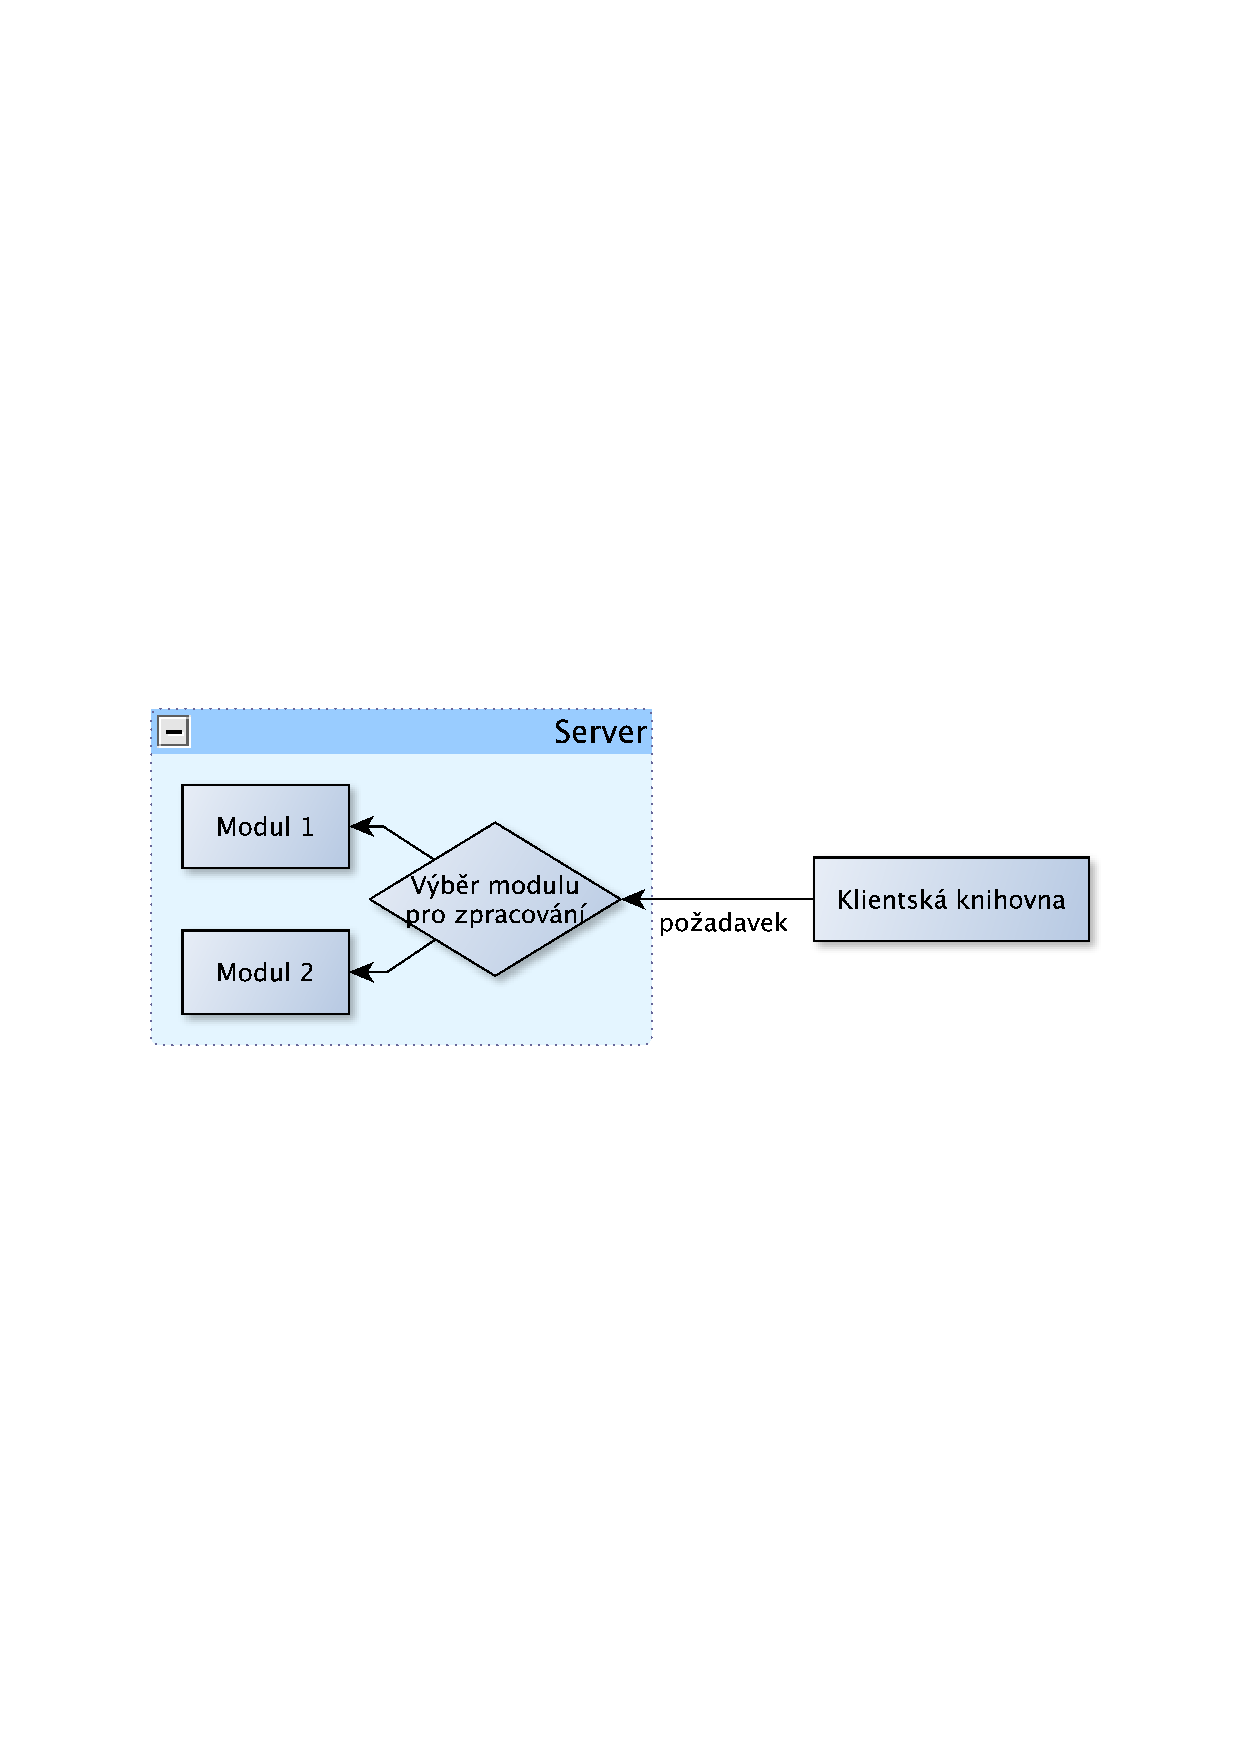
\includegraphics[trim=11cm 11cm 11cm 11cm, scale=0.7]{fig/navrh_moduly}
\caption{Návrh využití modulů.}
\label{fig:FigureExample}
\end{figure}

Jednotlivé moduly serveru jsou navrženy jako dynamické knihovny.
Při spuštění serveru jsou nahrány všechny moduly z adresáře nastavitelného pomocí konfiguračního souboru.

Každý modul obsahuje následující informace:

\begin{itemize}
\item \textbf{URI} - URI modulu, na kterém daný modul pracuje. Každý modul serveru musí mít své jedinečné URI.
\item \textbf{Typ} - Typ modulu. Všechny moduly daného typu poskytují stejné komunikační rozhraní. To umožňuje klientské knihovně
komunikovat i s pro ni neznámými moduly pouze na základě znalosti jejich typu.
\item \textbf{Popis} - Krátký text popisující funkci modulu. V grafickém rozhraní je tento text zobrazen v seznamu modulů.
\end{itemize}

V rámci této bakalářské práce existují moduly jen dvou typů:

\begin{itemize}
\item \textbf{CALLINFO} - Moduly tohoto typu poskytují rozličné informace (například polohu nebo jméno operátora)
na základě volací značky. Data jsou získávána z veřejně dostupných služeb, nebo z databáze uložené na serveru.
\item \textbf{DXCLUSTER} - Moduly typu DXCLUSTER poskytují informace (například frekvenci a polohu) o stanicích,
které aktuálně vysílají.
\end{itemize}

\subsubsection{Rozhraní modulů typu CALLINFO}

S moduly typu CALLINFO lze komunikovat následujícími způsoby:

\begin{itemize}
\item \textbf{Požadavek typu POST na URI "/modul"} - Jako data je v požadavku zaslána volací značka operátora. Odpověď obsahuje
veškeré zjistitelné informace o volací značce ve formátu CSV definovaném v podkapitole \ref{navrh_protokol}.
\item \textbf{Požadavek typu GET na URI "/modul/username"} - Pokud modul vyžaduje registraci uživatelského jména a hesla pro
přístup k databázi volacích značek (například v případě, že modul přistupuje ke službě, která je jen pro registrované), musí modul
implementovat zpracování tohoto URI a vrátit aktuálně registrované uživatelské jméno nebo prázdný řetezec. Klient pak může tohoto
chování využít pro zjištení, jestli je potřeba být pro použití modulu registrován.
\item \textbf{Požadavek na URI "/modul/register"} - Slouží k registraci uživatelského jména a hesla pro použití modulu.
Jméno a heslo jsou předány v hlavičce paketu pod klíči "username" a "password".
\end{itemize}

\subsubsection{Rozhraní modulů typu DXCLUSTER}

Moduly typu DXCLUSTER poskytují následující funkce:

\begin{itemize}
\item \textbf{Požadavek typu GET na URI "/modul"} - Modul vrátí seznam nově vysílajících stanic od posledního dotazu. Klient se tak
musí opakovaně ptát, aby získal nové vysílající stanice.
\item \textbf{Požadavek typu GET na URI "/modul/username"} - Význam je stejný jako u modulu typu CALLINFO.
\item \textbf{Požadavek na URI "/modul/register"} - Význam je stejný jako u modulu typu CALLINFO.
\end{itemize}

\subsection{Databáze}
\label{navrh_databaze}

Součástí serveru je rozhraní pro přístup k databázi. Veškerá data všech uživatelů jsou v této databázi uložena.
Návrh serveru počítá s využitím databáze jakéhokoliv typu (SQLite3, MySQL, PostgreSQL, \dots). Jednotlivé moduly
umí prostřednictvím databázového rozhraní s databází pracovat a spouštět nad ní prakticky jakékoliv dotazy.

Na následujícím obrázku je zobrazeno obecné schéma databáze použité pro uložení všech potřebných informací. Tabulky
z tohoto obrázku jsou pak dále stručně popsány.

\begin{figure}[h]
\centering
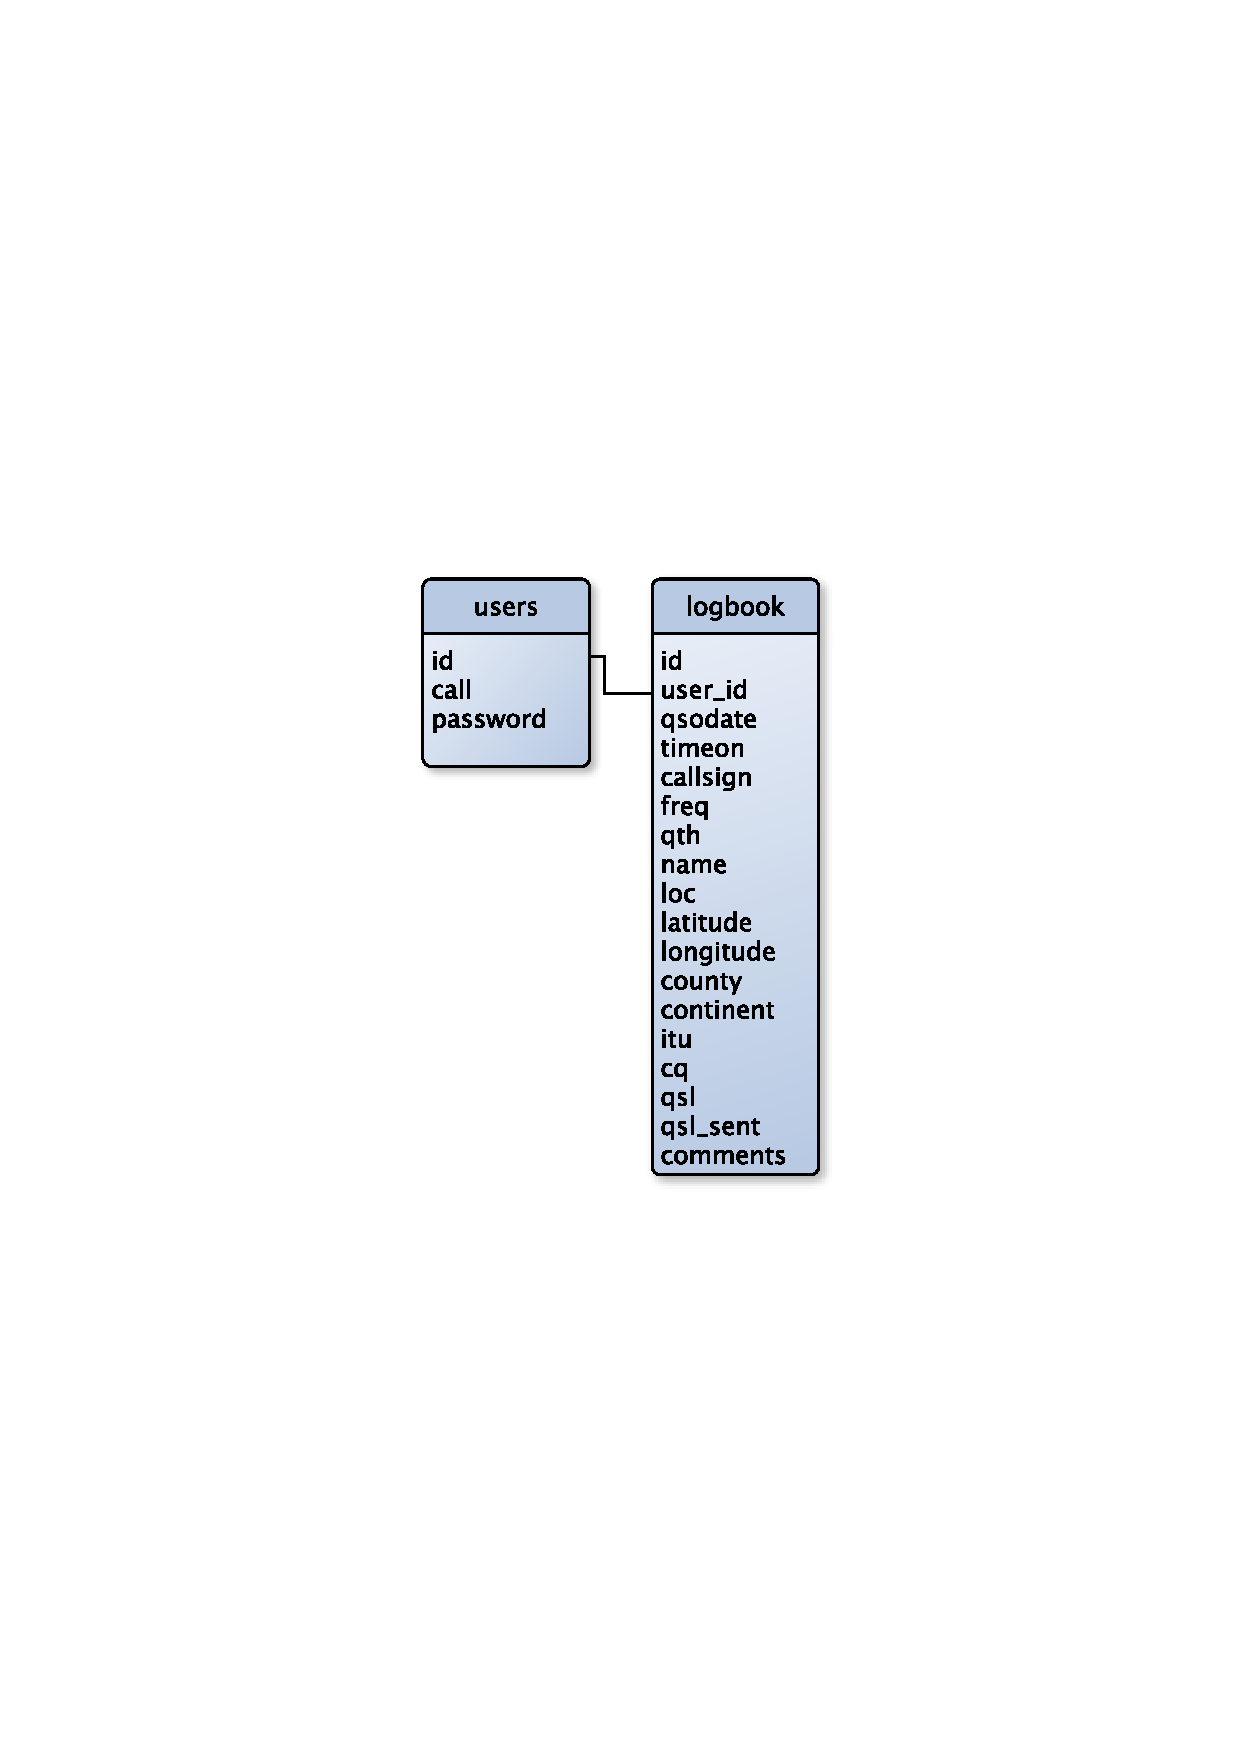
\includegraphics[trim=9cm 9cm 9cm 9cm, scale=0.7]{fig/navrh_databaze}
\caption{Návrh databáze.}
\label{fig:FigureExample}
\end{figure}

\subsubsection{Tabulka users}

Tabulka users obsahuje informace potřebné pro přihlášení uživatele deníku. Jde zejména o jeho volací značku a
heslo.

\subsubsection{Tabulka logbook}

V tabulce logbook jsou uloženy deníky všech uživatelů. Obsahuje následující sloupce:

\begin{itemize}
\item \textbf{id} - ID záznamu v logu.
\item \textbf{user\_id} - ID uživatele, jemuž záznam v logu patří.
\item \textbf{qsodate} - Datum záznamu ve formátu unixového timestampu.
\item \textbf{callsign} - Volací značka (například OK2JRQ).
\item \textbf{mode} - Mód spojení.
\item \textbf{qth} - QTH lokátor (Maidenhead Locator).
\item \textbf{name} - Jméno operátora.
\item \textbf{latitude} - Zeměpisná šířka.
\item \textbf{longitude} - Zeměpisná délka.
\item \textbf{conty} - Okres.
\item \textbf{continent} - Zkratka kontinentu.
\item \textbf{cq} - CQ zóna.
\item \textbf{itu} - ITU zóna.
\item \textbf{qsl} - Příznak žádosti o QSL lístek.
\item \textbf{qsl\_sent} - Příznak poslání QSL lístku.
\item \textbf{comments} - Komentáře.
\end{itemize}

\section{Klientská knihovna}
\label{navrh_knihovna}

Cílem klientské knihovny je poskytnout grafickému rozhraní jednotné API pro přístup k serveru
a tím pádem zamezit duplikování kódu mezi případnými grafickými rozhraními.

Klientská knihovna má minimální závislosti a je multiplatformní. Pomocí komunikačního protokolu
komunikuje se server, zpracovává příchozí data a předává je klientovi.

Knihovna je navržena tak, aby mohla spolupracovat s jakýmkoliv grafickým rozhraním.

Základními funkcemi klientské knihovny je:

\begin{itemize}
\item Připojení k serveru, registrace a přihlášení uživatele.
\item Generování požadavků pro server a jejich posílání.
\item Zpracování odpovědí serveru a předání zpracovaných dat klientské knihovně.
\end{itemize}

\section{Klient}
\label{navrh_klient}

Klient slouží koncovému uživateli k připojení k serveru, prezentaci aktuálních dat a jejich změně. Pro komunikace
se serverem klient využívá klientskou knihovnu. Pro komunikaci s uživatelem pak klient využívá grafického rozhraní.
Po startu klienta je uživatel vyzván k přihlášení se k serveru. Uživateli je rovněž nabídnuta možnost registrace
nového účtu.

Po přihlášení zobrazí klientská aplikace veškeré záznamy v deníku a umožní jejich editaci. Klientská aplikace také zobrazuje
aktuální vysílání získané ze služby DXCluster. Stanice, které aktuálně vysílají jsou zobrazeny graficky na modelu zeměkoule.

Po vybrání stanice zobrazen dialog pro přidání nového záznamu s předvolenými hodnotami získanými ze služby DXCluster. Automaticky
je také přeladěno rádio na danou frekvenci. V okně pro nový záznam je uživateli zobrazena historie všech spojení s daným operátorem.
Po potvrzení dialogu je nový záznam odeslán na server a uložen do databáze.

Klient také umožňuje zobrazit všechny moduly dostupné na serveru a jejich popis.


\chapter{Implementace}
\label{implementace}

V této kapitole je popsána implementace serverové aplikace, klientské aplikace a klientské knihovny.

\section{Implementace serverové aplikace}
\label{implementace_server}

Server byl implementován v jazyce C++ umožňujícím lepší dekompozici aplikace a použití objektového paradigmatu. Byla rovněž
použita knihovna Boost, která poskytuje základní metody pro asynchronní síťovou komunikaci a nabízí programátorské prostředky
nad rámec standardní STL knihovny.

Pro implementaci modulu QRZ bylo potřeba použít knihovnu pro zpracování XML. K tomuto účelu jsem použil knihovnu TinyXML.

V této podkapitole jsou popsány nejdůležitejší třídy serveru.

\subsubsection{Třída Server}

Třída Server je základní třídou serveru. Vytváří soket, na kterém server přijímá připojení z klientské knihovny. Jakmile je 
akceptováno nové připojení, je vytvořena instance třídy Session, která dále zpracovává všechny požadavky klienta.

\subsubsection{Třída Session}

Tato třída reprezentuje sezení jednoho uživatele. Při obdržení nových dat od klienta jsou tato předána instanci třídy
RequestParser, která slouží k jejich rozparsování. Pokud byla obdržena kompletní zpráva, je předána instanci třídy 
ModuleManager metodou handleRequest, která pak řídí její další zpracování. Výsledná odpověď je pak třídou Session poslána
zpět klientovi.

\subsubsection{Třída RequestParser}

Třída RequestParser reprezentuje konečný automat pro parsování zpráv podle specifikace komunikačního protokolu.
Metoda parse zpracovává přijatá data, parsuje je, a výsledek uchovává v instanci třídy Request. Pokud dojde během parsování
k chybě, vrací funkce parse hodnotu false a uživatel, jehož klient poslal nevalidní data, je odpojen.

\subsection{Implementace databázového rozhraní}
\label{implementace_db}

Návrh a implementace serveru umožňuje použití libovolného databázového rozhraní. V rámci bakalářské práce je však podpována
pouze databáze SQLite3. Třída implementující konkrétní databázové rozhraní musí dědit třídu StorageBackend a implementovat
její čistě virtuální metody.

\begin{figure}[h]
\centering
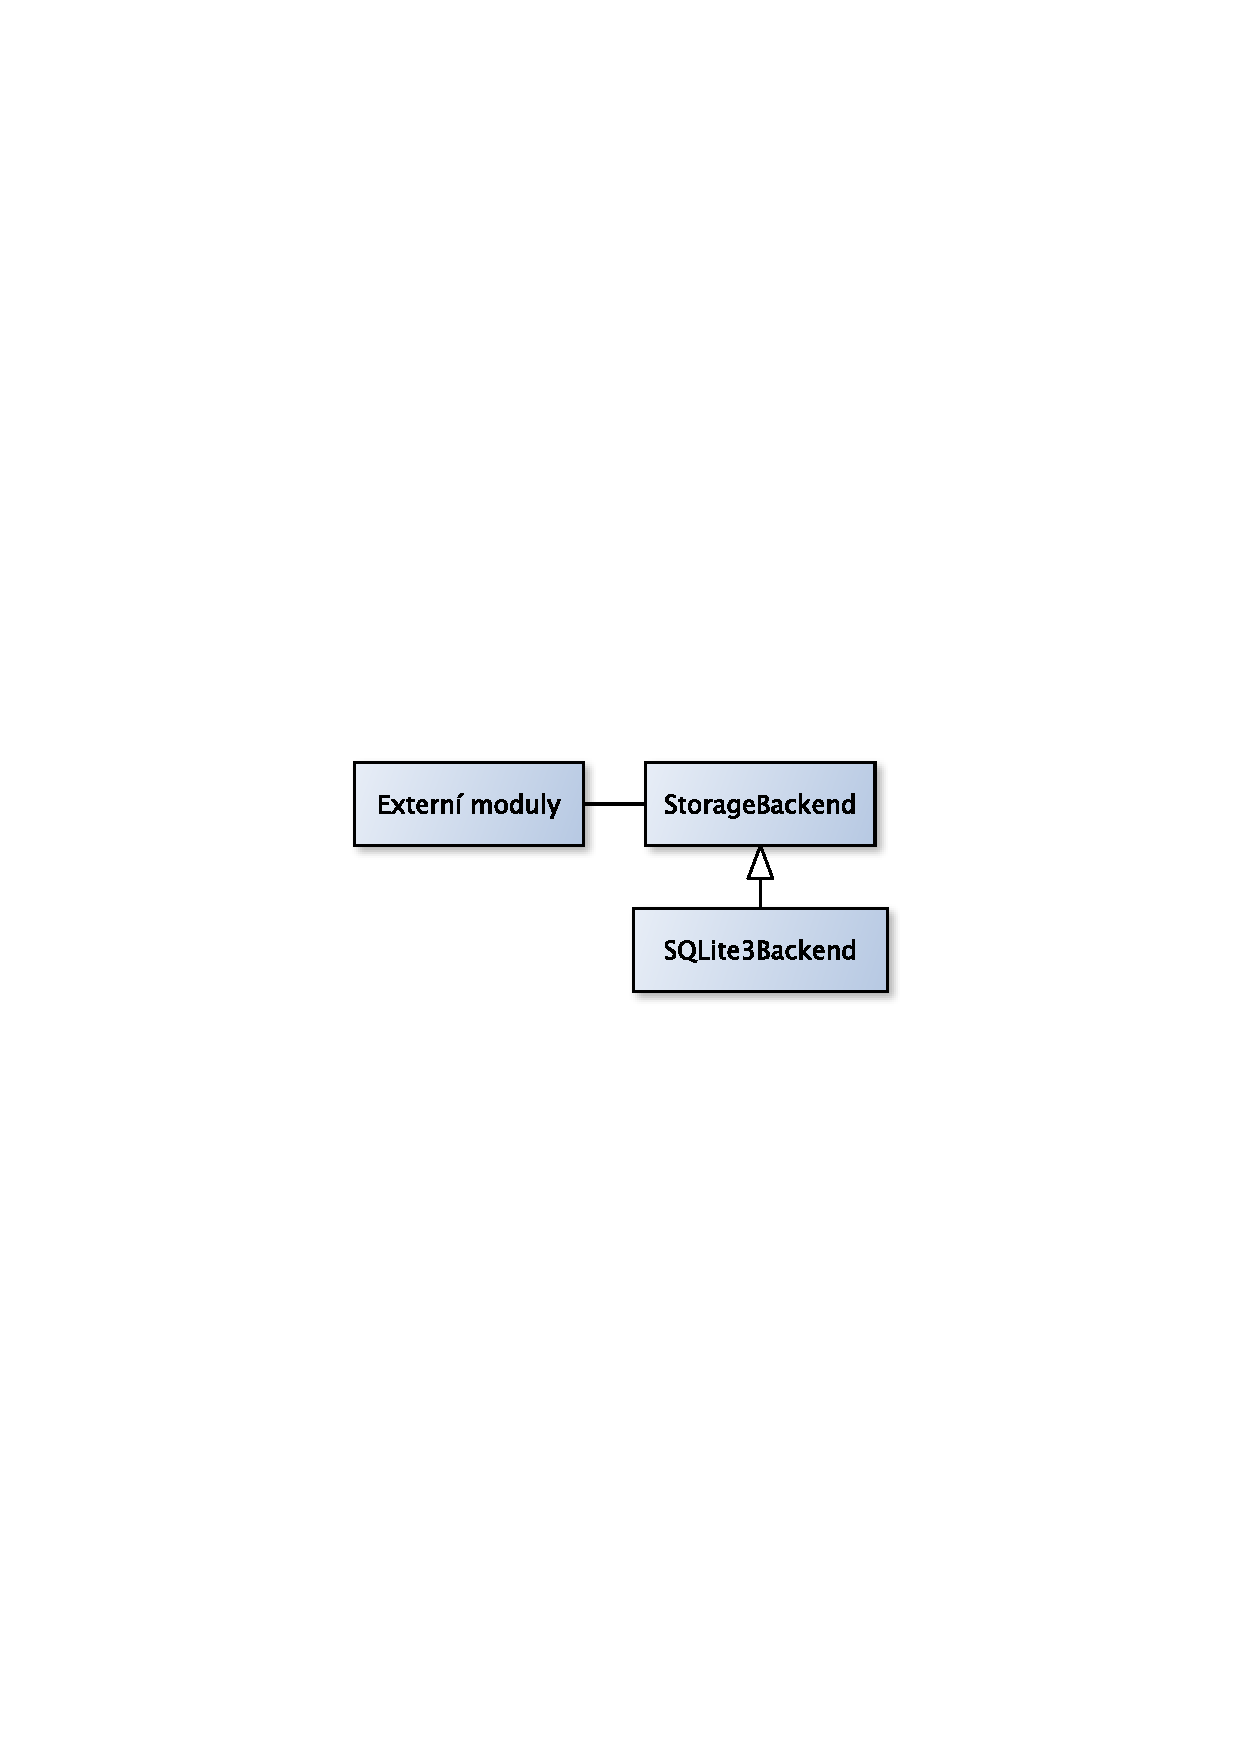
\includegraphics[trim=12cm 12cm 12cm 12cm, scale=0.7]{fig/imp_databaze}
\caption{Diagram databázového rozhraní.}
\label{fig:FigureExample}
\end{figure}

\subsubsection{Třída StorageBackend}

Třída StorageBackend je základní abstraktní třídou pro implementaci jakéhokoliv databázového rozhraní.
Je u ní použit návrhový vzor Singleton a jejím smyslem je poskytnout rozhraní pro získávání dat z databázového rozhraní bez znalosti
o jakou databázi se jedná. Názvy metod a podtříd jsou pojmenovány terminologií známou z SQL databází, ale prakticky
lze pomocí třídy StorageBackend implementovat rozhraní pro přístup k jakémukoliv typu databáze.

Třída StorageBackend Obsahuje základní podtřídy pro definici dotazů typu SELECT, INSERT, UPDATE a CREATE známých z
jazyka SQL:

\begin{itemize}
\item StorageBackend::Column - Obsahuje veškeré informace o sloupci tabulky (jméno, typ, velikost,
příznaky pro NOT NULL, UNIQUE a PRIMARY KEY). Slouží pro definici sloupce při vytváření
nové tabulky metodou StorageBackend::createTable().
\item StorageBackend::Select - Zapouzdřuje data potřebná pro provedení výběru dat z databáze. Obsahuje jméno tabulky,
ze které se výběr provádí, a ukazatel na dvourozměrně pole, do kterého se uloží výsledky. Dále umožňuje třída StorageBackend::Select
definovat omezení výběru (v SQL jazyce klíčové slovo WHERE) a umožňuje výběr konkrétních sloupců, které vrátí ve výsledku.
Instance této třídy je předána metodě StorageBackend::select() nebo StorageBackend::remove().
\item StorageBackend::Insert - Obsahuje data pro vložení (v SQL jazyce INSERT) nebo aktualizaci (v SQL jazyce UPDATE)
záznamu v databázi. Obsahuje název tabulky, ve které se budou data měnit, a samotná data ve formě název sloupce - hodnota.
Umožňuje definovat omezení (v SQL jazyce WHERE) aplikovaná při aktualizaci dat. Instance této třidy je předána metodě
StorageBackend::insert() nebo StorageBackend::update().
\end{itemize}

V závislosti na implementaci metod třídy StorageBackend v něktéré z jejich dceřiných tříd je pak vyvolána konkrétní změna v
databázi. Třída StorageBackend dále umožňuje získání identifikačního čísla naposledy vloženého záznamu metodou lastInsertedID().


\subsubsection{Třída SQLite3Backend}

Tato třída dědí třídu StorageBackend a implementuje její metody pro použití databázového systému SQLite3. V metodách
update(), insert(), select(), createTable() a remove() se na základě předaných dat vygeneruje dotaz v SQL jazyce, spustí se
a je vrácen výsledek.

\subsection{Implementace modulů}
\label{implementace_moduly}

Moduly jsou implementovány jako dynamické knihovny. Každý modul musí dědit třídu Modul (zprostředkovaně například přes třídu RequestResponder)
a implementovat její čistě virtuální
(pure virtual) metody. Veškeré klientské požadavky jsou pak směrovány na konkrétní modul podle URI instancí třídy ModuleManager.

\begin{figure}[h]
\centering
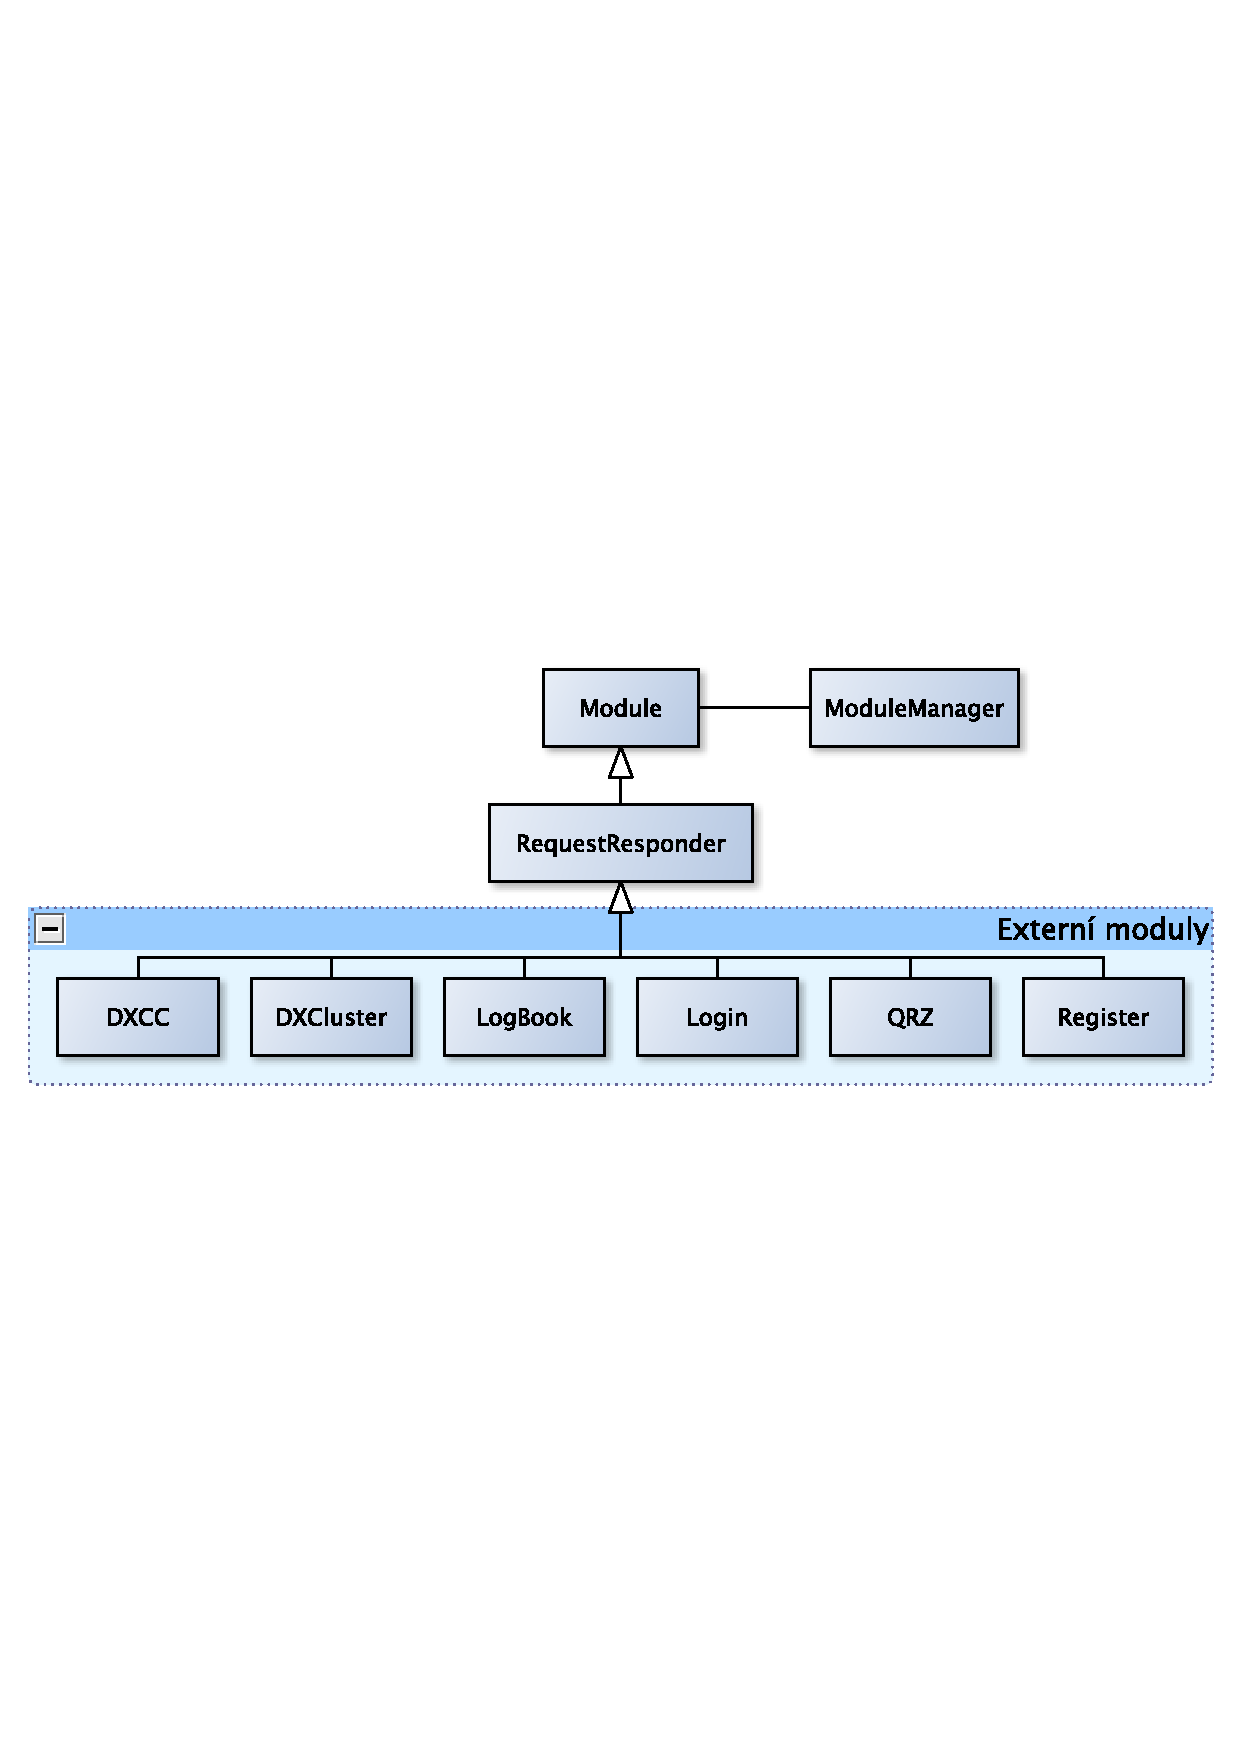
\includegraphics[trim=10cm 10cm 10cm 10cm, scale=0.7]{fig/moduly}
\caption{Diagram tříd modulů.}
\label{fig:FigureExample}
\end{figure}

\subsubsection{Třída Module}

Třída Module poskytuje základní třídu, kterou musí implementovat každý externí modul. Obsahuje základní informace o modulu 
(jeho jméno, typ a popis).

\subsubsection{Třída RequestResponder}

Tato třída dědí třídu Module a rozšiřuje ji o data a metody specifické pro modul odpovídající na klientské požadavky.
Přiřazuje modulu jeho URI a informaci o tom, jestli musí být uživatel pro jeho použití přihlášen.
Obsahuje také deklaraci metody handleRequest(), která je volána instancí třídy ModuleManager pro každý příchozí požadavek
smeřující na modul.

\subsubsection{Třída ModuleManager}

U třídy ModuleManager je použit návrhový vzor Singleton.
Tato třída zabezpečuje veškerou práci serveru s externími moduly. Pomocí 
metody loadModules lze načíst všechny moduly z adresáře zvoleného v konfiguračním souboru. Veškeré požadavky od klientů
jsou předány instanci této třídy metodou handleRequest, která je pak dále směruje podle URI na konkrétní modul. Třída také
umožňuje poslat seznam všech modulů klientské aplikaci.

\subsection{Seznam implementovaných modulů}
\label{implementace_moduly_list}

V této podkapitole jsou popsány jednotlivé implementované moduly.

\subsubsection{Modul Register}

Modul Register (běžící na URI "/register") slouží k registraci nových uživatelů. Při svém spuštění vytvoří pomocí
instance třídy StorageBackend tabulku "users". V metodě handleRequest pak přijímá případné požadavky na registraci
uživatele a přidá nového uživatele do databáze. Pokud je již uživatel zaregistrován, vrací klientské aplikaci chybový kód.

\subsubsection{Modul Login}

Modul Login běží na URI "/login". Jeho cílem je umožnit uživatelům přihlášení k systému. V metodě handleRequest je
implementován princip přihlášení WWW-Authenticate.

\subsubsection{Modul LogBook}

Tento modul je základem celého projektu, protože umožňuje uživateli ukládat nové záznamy v deníku na server. Při svém načtení
vytvoří tabulku "logbook". V metodě handleRequest na základě URI provádí následující akce:

\begin{itemize}
\item URI "/logbook" - Jako odpověd na dotaz pošle celý logbook v CSV formátu získaný z databáze pomocí instance třídy StorageBackend.
\item URI "/logbook/add" - Přidá do tabulky "logbook" nový záznam podle CSV dat přijatých v dotazu.
\item URI "/logbook/remove" - Odstraní z tabulky "logbook" záznam definovaný pomocí ID přijatého v dotazu.
\item URI "/logbook/call" - Jako odpověď na dotaz pošle pouze záznamy o spojeních s konkrétním operátorem určeným jeho značkou v 
těle dotazu.
\end{itemize}

\subsubsection{Modul DXCC}

Modul DXCC (běží na URI "/dxcc") umožňuje získat z volací značky bližší informace o její lokaci. Modul je typu CALLINFO.
Data o jednotlivých prefixech
jsou po startu modulu načtena ze souboru "cty.csv" v CSV formátu. Tento soubor byl získán z TODO.
V metodě handleRequest modul získá z požadavku prefix volací
značky, vyhledá jej v datech načtených při startu a jako odpověď odešle informace o lokaci stanice. Pokud prefix není nalezen,
vrací chybový kód.

\subsubsection{Modul DXCluster}

Modul DXCluster (běžící na URI "/dxcluster") slouží k připojení k DXClusteru dxspots.com. Modul je typu DXCLUSTER.
Při prvním požadavku od klienta dojde k připojení na DXCluster.
Veškerá data přijatá z DXClusteru jsou rozparsována a uložena v CSV formátu. Na každý
další klientský požadavek odpoví modul daty získanými z DXClusteru. Jde tedy o jistou formu pollingu, kdy si klient
opakovaně žádá o nová data.

\subsubsection{Modul QRZ}

Modul QRZ (běžící na URI "/qrz") je typu CALLINFO umožňuje tedy získávat uživateli další informace o ostatních uživatelích na základě jejich
volací značky.K tomuto využívá službu qrz.com. V metodě handleRequest se na základě URI provádí následující akce:

\begin{itemize}
\item URI "/qrz" - Pošle QRZ serveru požadavek pro získání informací o uživateli na základě jeho volací značky. Ke komunikaci 
s QRZ serverem je využíváno XML API, které tento server poskytuje. Odpověď na požadavek je rozparsována pomocí knihovny 
TinyXML a odeslána klientské aplikaci ve formátu CSV.
\item URI "/qrz/register" - Umožňuje uživateli zvolení nebo změnu hesla použitého pro přihlášení k QRZ serveru.
\end{itemize}

Komunikace se serverem QRZ je rovněž asynchronní a odpověď na dotaz na QRZ modul není odeslána ihned.
Je tak třeba řešit problém, kdy klientská aplikace pošle dotaz na QRZ modul
následovaný dotazem na modul jiný. V tomto případě by mohl být druhý dotaz zpracován před prvním a došlo by tak k narušení
způsobu komunikace dotaz-odpověď.

Řešením tohoto problému je možnost modulu zastavit dočasně zpravovávání dalších požadavků od konkrétního klienta, dokud 
nebude vyřízen požadavek aktuální. To lze provést zavoláním metody Reply::setAsync(). Jakmile je odpověď připravena
k odeslání, lze ji odeslat metodou Session::sendAsyncReply(). Po zavolání této metody je pak opět povoleno zpracovávání
dalších požadavků od klienta.

\subsubsection{Modul Hamlib}

Modul Hamlib (běžící na URI "/hamlib") umožňuje ovládat frekvenci vysílačky připojené k počítačí, na které
běží serverová aplikace. Pro změnu a získání frekvence využívá knihovnu Libhamlib. V metodě handleRequest se na základě
URI provádí tyto akce:

\begin{itemize}
\item dotaz typu POST na URI "/hamlib" - Přeladí frekvenci vysílačky na frekvenci získanou z požadavku. Frekvence
je posílána jako desetinné číslo v kHz.
\item dotaz typu POST na URI "/hamlib" - Odešle zpět aktuální frekvenci jako desetinné číslo v kHz.
\end{itemize}

\subsection{Implementace logování}
\label{implementace_logovani}

Logování je implementováno s použitím knihovny Log4cxx vyvíjené Apache Software Foundation a licencované pod licencí
Apache License. Pokud však není při kompilaci knihovna Log4cxx nalezena, je pro logování použit standardní výstup.
Výhodou Použití Log4cxx je možnost široké konfigurace logování pomoci konfiguračního souboru, možnost přesměrovat
logování do souboru a tento pak automaticky rotovat na základě jeho velikosti nebo času.

Každá třída serveru má vlastní statickou instanci třídy log4cxx::LoggerPtr, kterou využívá k logování.
U každého zápisu do logu se loguje datum a čas, závažnost záznamu (Informace, varování, chyba), název modulu a samotný
logovaný záznam.S tandardní výstup pak vypadá například následovně:

\begin{verbatim}
2012-03-28 19:12:44,423 INFO  Server: Starting the server
\end{verbatim}

\section{Implementace klientské knihovny}
\label{implementace_knihovna}

Klientská knihovna spojuje serverovou aplikaci se samotným klientským rozhraním.
Klientská knihovna je navržena a implementována
tak, aby ji bylo možno použít s jakýmkoliv grafickým (případně i konzolovým) rozhraním. Kvůli přenositelnosti a
širší využitelnosti je napsána v jazyce C s důrazem na co nejméně závislostí na jiných knihovnách.

Klientská knihovna je rozdělena do menších bloků, které budou v této kapitole postupně popsány.

\subsection{Abstraktní datové typy}

V této podkapitole je popsána implementace abstraktních datových typů požitých v klientské knihovně.

\subsubsection{HAMList - Seznam}

\begin{figure}[h]
\centering
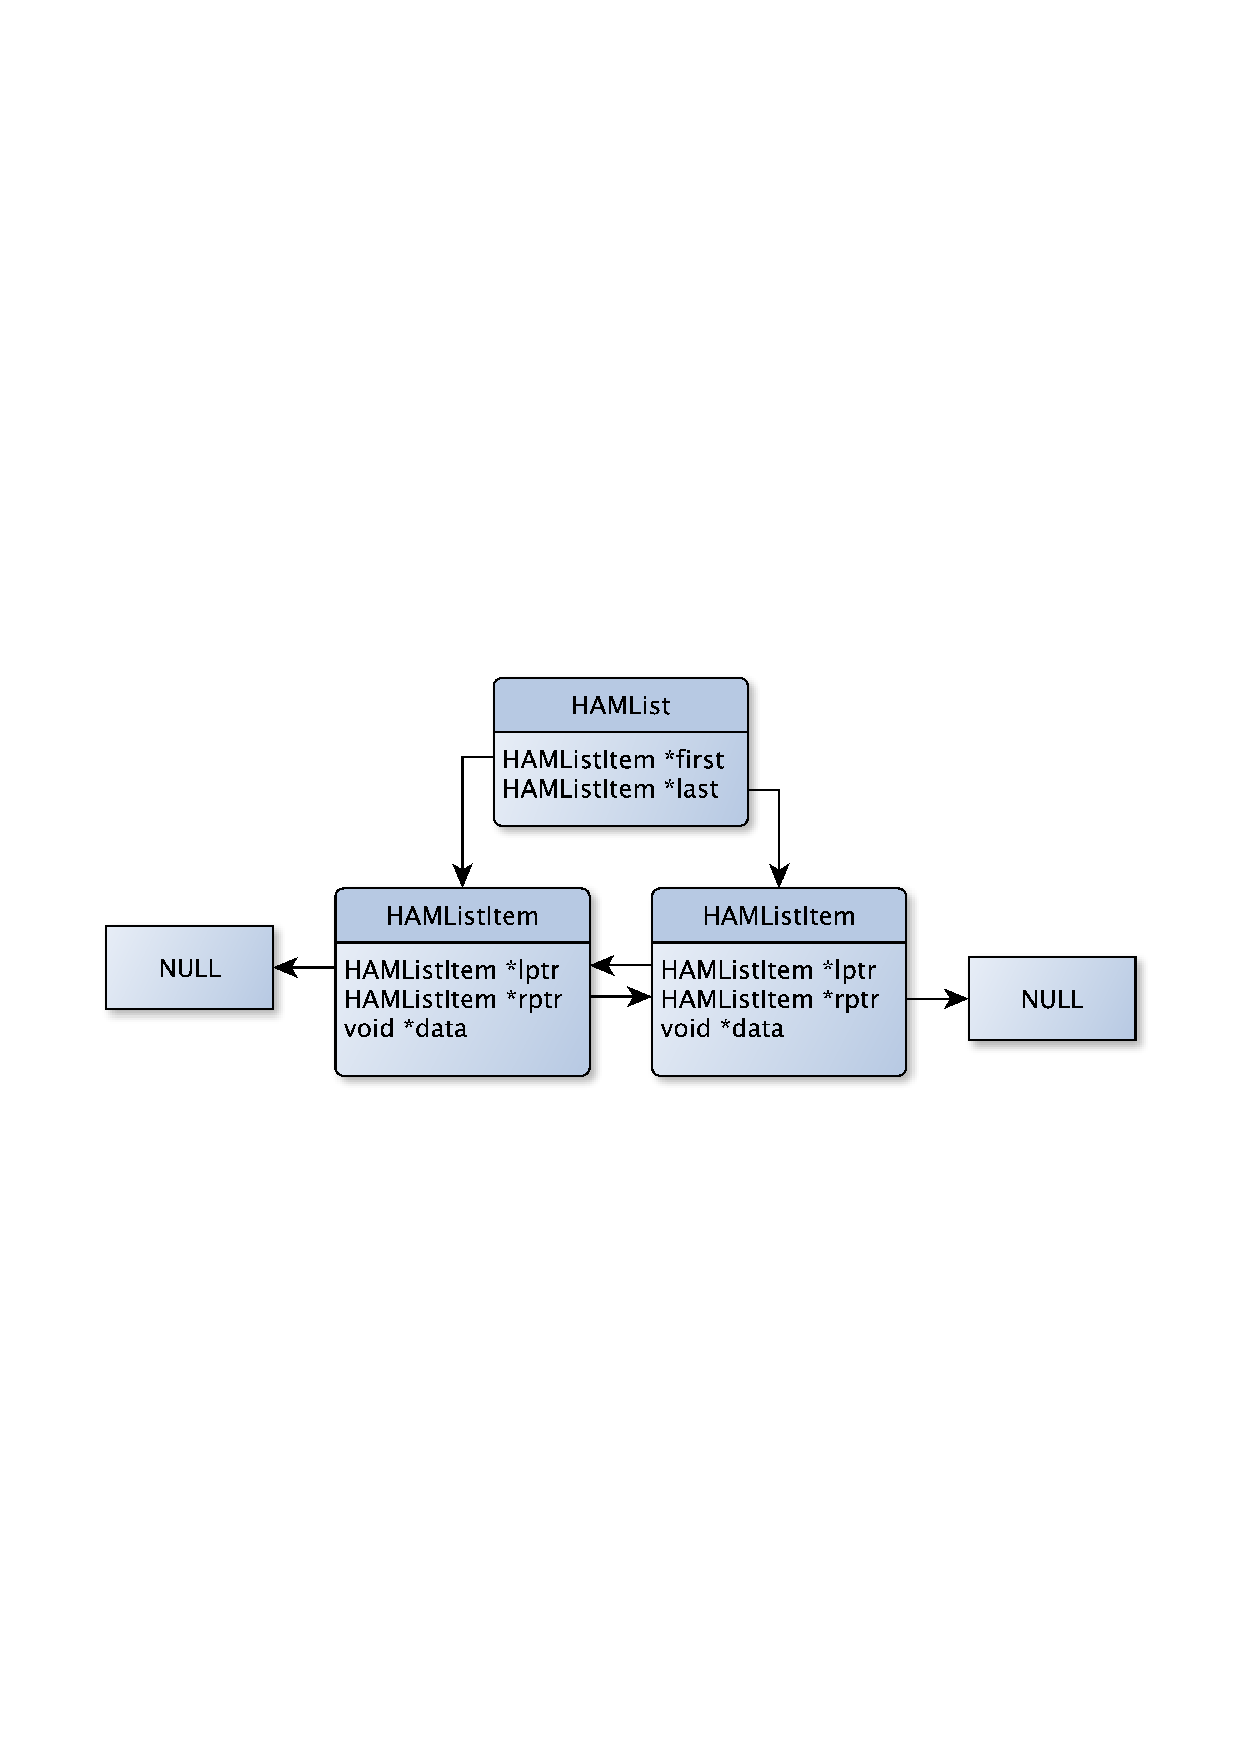
\includegraphics[trim=8cm 8cm 8cm 8cm, scale=0.6]{fig/list}
\caption{Diagram dvousměrného seznamu.}
\label{fig:FigureExample}
\end{figure}

HAMList je implementací dvousměrného seznamu. Základní datové struktury použité pro definici seznamu jsou
HAMList a HAMListItem:

\begin{verbatim}
typedef struct _HAMListItem {
	void *data;
	struct _HAMListItem *lptr;
	struct _HAMListItem *rptr;
} HAMListItem;

typedef struct _HAMList {
	HAMListItem *first;
	HAMListItem *last;
	HAMListItemDataFree free_func;
} HAMList;
\end{verbatim}

Každá položka HAMListItem obsahuje odkaz na svého předchůdce (lptr) a následníka (rptr) a samotná data spjatá
s položkou (data). Struktura HAMList obsahuje odkaz na první a poslední položku a ukazatel na funkci free\_func,
která je použita pro uvolnění uživatelských dat z paměti. Pokud není tato funkce definována, nejsou uživatelská
data při uvolňování seznamu z paměti uvolněna.

\subsubsection{HAMHashTable - Hashovací tabulka}

\begin{figure}[h]
\centering
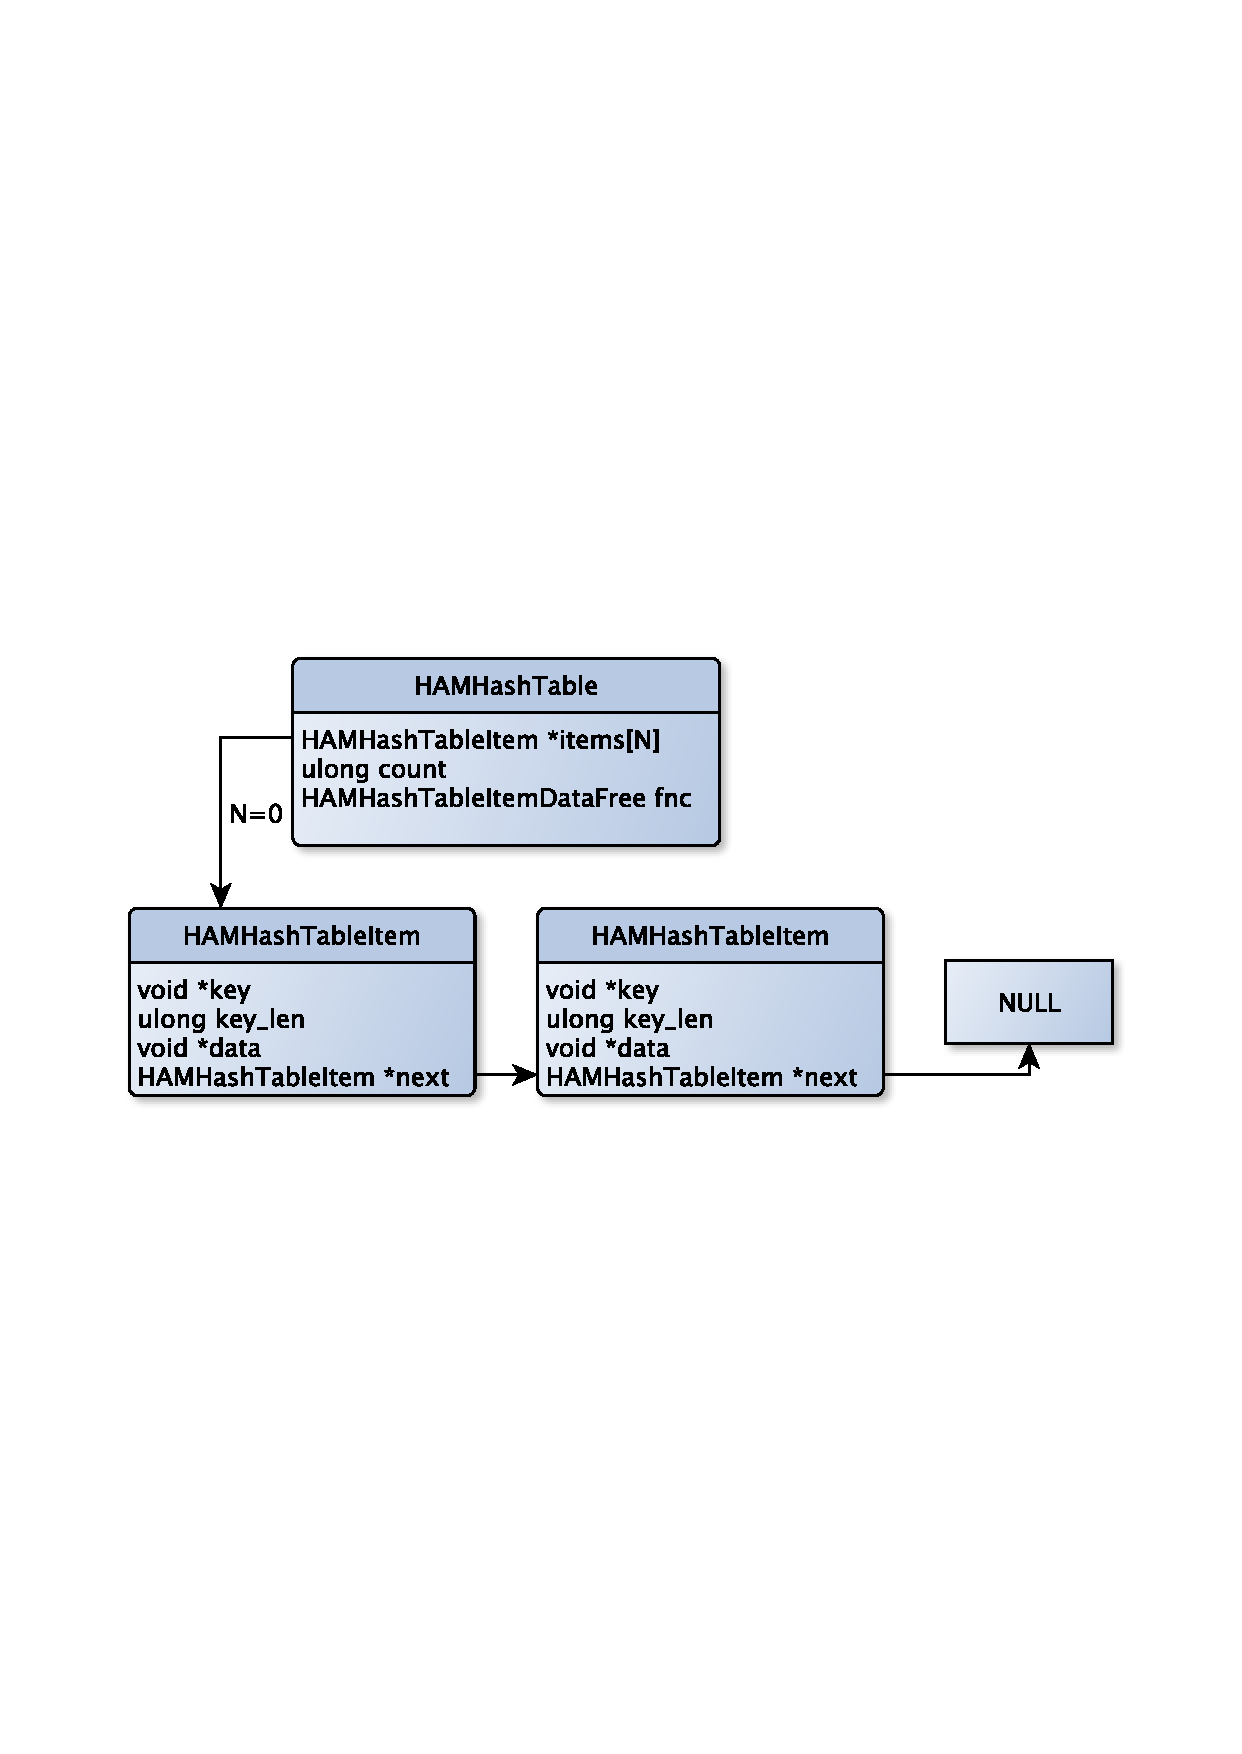
\includegraphics[trim=8cm 8cm 8cm 8cm, scale=0.6]{fig/hash}
\caption{Diagram hash tabulky seznamu.}
\label{fig:FigureExample}
\end{figure}

HAMHashTable je implementací hash tabulky. Základní datové struktury použíté při implementaci hash tabulky jsou
HAMHashTableItem a HAMHashTable:

\begin{verbatim}
typedef struct _HAMHashTableItem {
	const void *key;
	void *data;
	unsigned long key_len;
	struct _HAMHashTableItem *next;
} HAMHashTableItem;

typedef struct _HAMHashTable {
	HAMHashTableItem *items[HAM_HASH_LEN];
	unsigned long count;
	HAMHashTableItemDataFree free_func;
} HAMHashTable;
\end{verbatim}

Každá položka uložená v hash tabulce obsahuje svůj klíč (key), jeho délku (key\_len), data svázaná s položkou a ukazatel
na další položku. Při vložení nové položky do tabulky je vypočten hash jejího kliče pomocí SDBM hashovacího algoritmu.
Na základě hodnoty hashe je ukazatel na položku uložen do pole položek items. P

\subsection{Komunikace s klientskou aplikací}
\label{implementace_knihovna_komunikace}

Pro komunikaci s klientskou aplikací je podstatné napojení na její smyčku událostí a možnost předávat asynchronně
výsledky požadavků odeslaných serveru. V této podkapitole jsou popsány řešení obou těchto problémů

\subsubsection{EventLoop}

Eventloop (neboli smyčka událostí) sdružuje metody sloužící k napojení na hlavní smyčku
klientské aplikace. Pro správnou funkci klientské
knihovny musí klientská aplikace implementovat všechny funkce definované ve struktuře HAMEventLoopUICallbacks a
předat je klientské knihovně prostřednictvím metody ham\_eventloop\_set\_ui\_callbacks().

Funkce definované ve struktuře HAMEventLoopUICallbacks jsou pak používány dalšími částmi klientské knihovny na
následující činnosti:

\begin{itemize}
\item timeout\_add - Přidá do hlavní smyčky programu běžící v klientské aplikaci nový časocač. Klientská aplikace
musí vrátit ukazatel na strukturu jednoznačně identifikující časovač a
volat opakovaně funkci předánou jakou ukazatel ve zvoleném intervalu.
\item timeout\_remove - Odebere z hlavní smyčky časovač na základě jeho ukazatele na strukturu, která jej identifikuje.
\item input\_add - Přidá do hlavní smyčky klientské aplikace ukazatel na funkci, která je volána když jsou k dispozici
nová data na definovaném soketu. Klientská aplikace
musí vrátit ukazatel na strukturu jednoznačně identifikující tuto událost.
\item input\_remove - Odebere z hlavní smyčky ukazatel na funkci vstupu na
základě ukazatele na strukturu, která jej identifikuje.
\end{itemize}

Díky této abstrakci je tak možno napojit klientskou knihovnu na jakoukoliv smyčku událostí.

\subsubsection{Signály}

Jednotlivé části klientské knihovny umožňují definovat signály, na které se pak může klientská aplikace napojit.
Seznam signálů je uložen v hash tabulce, kde klíčem je název signálu a daty seznam funkcí, které jsou zavolány
pokud je signál emitován. K registraci nových signálů slouží funkce ham\_signals\_register\_signal().

Klientské aplikaci je umožněno funkcí ham\_signals\_register\_handler() zaregistrovat funkci, která je zavolána
při emitování signálu. Funkce musí být ve formátu HAMFetchHandler. Při registraci signálu lze rovněž definovat
ukazatel na data, která jsou při emitování signálu zpracovávající funkci předána. Toho lze využít pro udržování
kontextu při zpracovávání signálu.


\subsection{Komunikace se serverem}

Tato podkapitola popisuje implementaci komunikace se serverem v klientské knihovně. Je zde popsáno rozhraní pro
připojení k serveru, parser komunikačního protokolu a pomocné struktury Reply a Request pro reprezetanci odchozích a
příchozích paketů.

\subsubsection{Připojení k serveru}

Pro připojení k serveru je nutné vytvořit novou instanci struktury Connection funkcí ham\_connection\_new(). Touto funkcí
se definuje adresa a port serveru, uživatelské jméno a heslo. Samotné připojení proběhne až po zavolání funkce
ham\_connection\_connect(). Tato funkce vytvoří nový soket pro připojení k serveru a pomocí funkce ham\_eventloop\_input\_add()
přidá do hlavní smyčky programu ukazatel na funkci pro parsování přijatých dat.

\subsubsection{Parsování dat}

K parsování dat v klientské knihovně slouží HAMParser. Ten funguje na stejném principu jako RequestParser na straně serveru.
Parsovaná data jsou ukládána do struktury Reply, která pak předána prostřednictvím signálu nebo zpětného volání (callbacku)
funkci, která požadavek na server iniciovala.

\section{Implementace klientské aplikace}
\label{implementace_klient}

Referenční klientská aplikace byla naprogramována v jazyce C++ s využitím grafického frameworku Qt. V této kapitole jsou stručně
popsány jednotlivé části klientské aplikace, třídy, které klientskou aplikaci implementují a jejich napojení na klientskou knihovnu.

\subsection{Hlavní okno programu}

V této podkapitole je popsána implementace hlavního okno programu a všech prvků, které jej tvoří.

\begin{figure}[h]
\centering
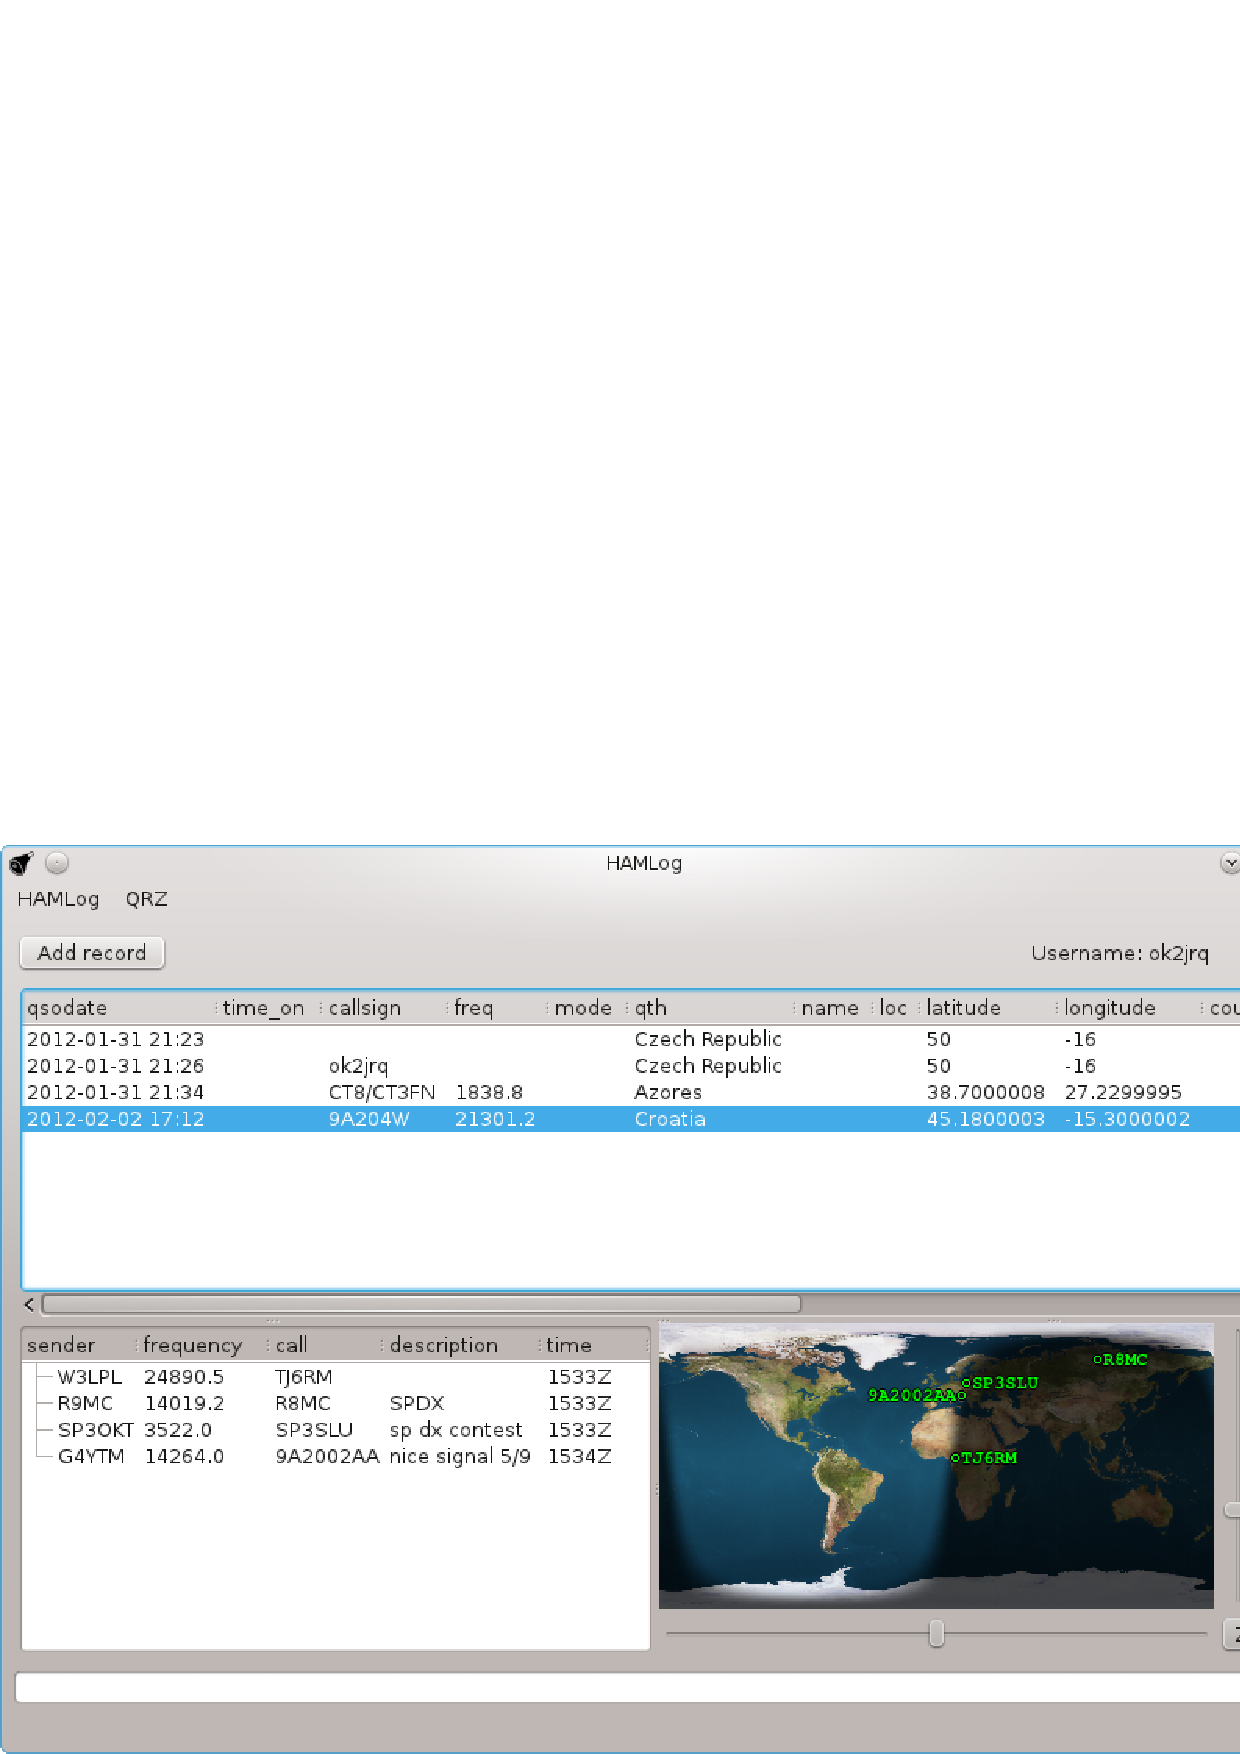
\includegraphics[trim=0cm 0cm 0cm 0cm, scale=0.7]{fig/ham3}
\caption{Hlavní okno aplikace.}
\label{fig:FigureExample}
\end{figure}

\subsubsection{Třída MainWindow}

Třída MainWindow reprezentující hlavní okno je také hlavní třídou klientské aplikace. Po svém vytvoření zobrazí dialog
pro připojení uživatele k serveru. Pomocí metody connectServer() se pak přihlásí k serveru. Registrovat nový uživatelský
účet lze metodou registerAccount.

Třída MainWindow se o úspěšném, případně neúspěšném přihlášení k serveru dozví díky napojení
na patřičné signály klientské knihovny. V této třídě je také obstarána komunikace mezi jednotlivými prvky tvořícími hlavní okno
prostřednictvím Qt signálů.

\subsubsection{Třída LogbookTreeWidget}

Třídou LogbookTreeWidget je uživateli umožněno zobrazení a editace logu prostřednictvím rozhraní podobného tabulce.
Je implementována nad Qt třídou QTreeWidget a komunikuje 
se serverovým modulem Logbook prostřednictvím klientské knihovny. Jednotlivé položky jsou editovatelné a změny se přenášejí
na server. Pokud uživatel poklepe na některou z položek, je zpracován příslušný Qt signál a otevřen dialog NewRecordDialog,
ve kterém může uživatel položku také editovat.

\subsubsection{Třída EarthWidget}

Třída EarthWidget je technologicky nejzajímavější třídou klientské aplikace. Umožňuje zobrazit zeměkouli promítnutou do roviny i 
formou klasického globusu. Na zeměkouli lze pak zobrazovat značky s popisky. Toho je využito pro zobrazení polohy právě vysilájících
stanic.

\begin{figure}[h]
\centering
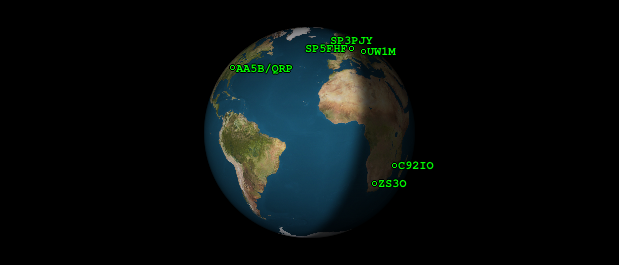
\includegraphics[trim=0cm 0cm 0cm 0cm, scale=0.9]{fig/ham5}
\caption{Ukázka možnosti zobrazení zeměkoule.}
\label{fig:FigureExample}
\end{figure}

Pro zobrazení zeměkoule je využita aplikace Xplanet. Při požadavku na překreslení okna je spuštěn nový proces Xplanet
s požadovanými parametry a je mu předáno ID widgetu, do kterého má vykreslovat. Značky s popisky jsou uloženy do dočasného souboru
a tento soubor je pak načten programem Xplanet a použit k vykreslení značek.
EarthWidget umožňuje také přiblížení na předdefinované lokace (například přiblížení Evropy) pomocí kontextového menu.

\subsubsection{Třída DXClusterWidget}

Pomocí třídy DXClusterWidget je zobrazen seznam aktuálně vysílajících stanic. Třída se prostřednictvím klientské knihovny
v pravidelných intervalech dotazuje
serveru na seznam aktuálně vysílajících stanic a tento pak zobrazuje. Pokud uživatel na některou ze stanic poklepe, otevře se 
dialog pro přidání nového záznamu. Seznam stanic je také předáván za pomoci Qt signálu třídě EarthWidget, která pak stanice
vykresluje na mapě.

\subsection{Přidání nového záznamu a editace}

Nový záznam lze přidat dvěma způsoby. Buď tak lze učinit pomocí tlačítka "Add Record" v hlavním okně programu, nebo poklepáním
na stanici získanou z DXClusteru. Obě možnosti pak vedou k vyvolání dialogu pro přidání nového záznamu. Stejný dialog je použit
také pro editaci již existujícího záznamu. Editaci lze vyvolat poklepáním na existující záznam v hlavním okně programu.

\begin{figure}[h]
\centering
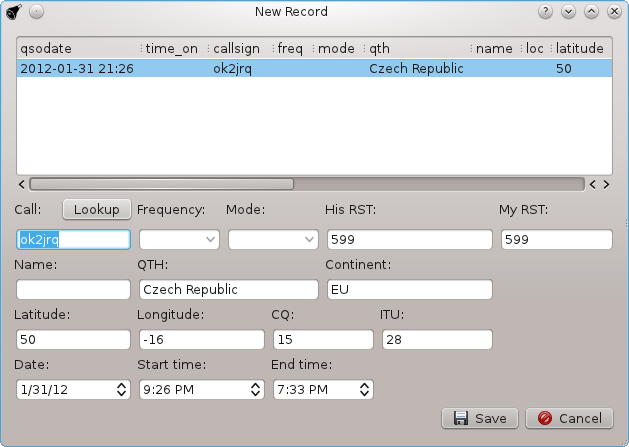
\includegraphics[trim=0cm 0cm 0cm 0cm, scale=0.9]{fig/ham4}
\caption{Dialog pro přidání a editaci záznamu.}
\label{fig:FigureExample}
\end{figure}

\subsubsection{Třída NewRecordDialog}

Dialog pro přidání nového záznamu a jeho editaci je implementován v třídě NewRecordDialog. Dialog se skládá ze dvou částí:

\begin{itemize}
\item Tabulka zobrazující předchozí spojení s přidávanou stanicí.
\item Formulář s jednotlivými poli o nově přidávaném záznamu.
\end{itemize}

Pro implementaci tabulky s předchozími spojeními je použita třída LogbookTreeWidget. Je tak znovu použit již jednou existující
kód.

V případě změny pole pro zadání volací značky (Call sign), je aktualizována tabulka s historií, a uživatel tak vidí předešlá 
spojení s danou stanicí. Také se pomocí klientské knihovny zjistí podrobné informace o zadané stanici a předvyplní se patřičná
pole. To zrychluje zadávání nových záznamu. V případě změny hodnoty v poli frekvence je na server odeslán požadavek o přeladění
rádia na zadanou frekvenci.

Po potvrzení dialogu jsou hodnoty všech polí prostřednictvím klientské knihovny přeneseny na server, kde jsou uchovány.

\subsection{Zobrazení dostupných modulů}

Dialog zobrazující moduly dostupné na server lze spustit prostřednictvím hlavního menu aplikace.

\begin{figure}[h]
\centering
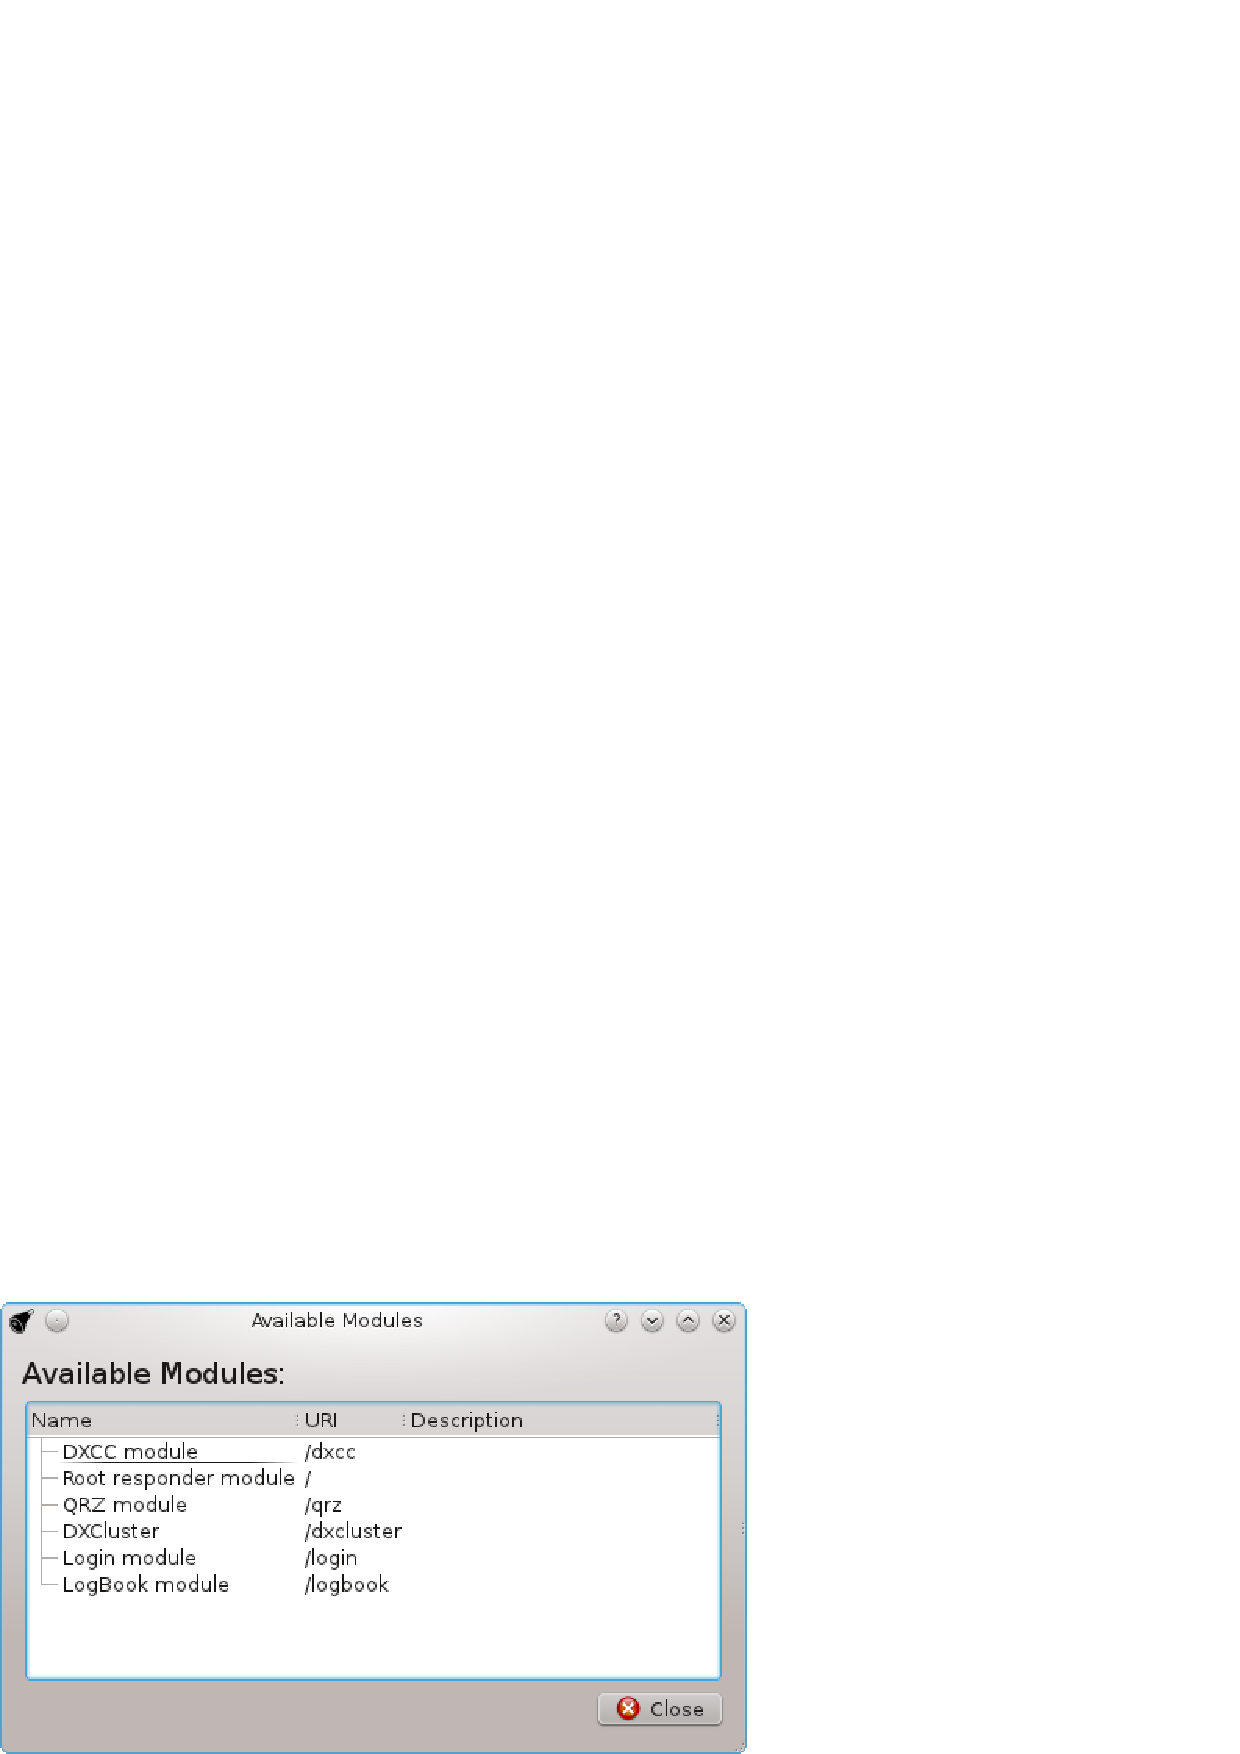
\includegraphics[trim=0cm 0cm 0cm 0cm, scale=1]{fig/ham6}
\caption{Dialog pro přidání a editaci záznamu.}
\label{fig:FigureExample}
\end{figure}

\subsubsection{Třída NewRecordDialog}

Dialog zobrazující dostupné moduly je implementován třídou NewRecordDialog. Jedná se o jednoduchou třídu, která pomocí
klientské knihovny získá ze serveru seznam modulů a zobrazí je formou tabulky vytvořené díky Qt widget QTreeWidget.


\chapter{Závěr}
Cílem této bakalářské práce bylo navhrnutí aplikace pro vedení staničního deníku pro použití radioamatéry. Důraz byl kladen zejména
na modularitu návrhu i výsledné implementance. Pro úspěšné dokončení práce bylo nejprve potřeba seznámit se s radioamatérským
hnutím a jeho fungováním a aplikacemi a metodami, které současní radiamatéři používají. K tomu bylo potřeba zorientovat se v 
radioamatérské technologii a pochopit fungování celého radioamatérského hnutí.
Výsledný návrh se rovněž snaží poučit z problémů současných aplikací a svou strukturou zaplnit volné místo mezi aplikacemi
umožňujícími vedení staničního deníku.

Výstupem implementace jsou tři oddělené projekty (serverová aplikace, klientská knihovna a grafické uživatelské rozhraní),
které spolu spolupracují a vzájemně se doplňují.

Serverová aplikace je plně modulární a umožňuje jednoduché přidávání nových
funkcí pomocí modulů. Splňuje veškeré požadavky na základní vedení staničního deníku (přidávání/editace záznamů, vyhledávání 
informací o ostatních radioamatérech nebo například ovládání vysílačky připojené k počítači).

Klientská knihovna je důležitým prvkem implementace, protože implementuje nízkoúrovňovou komunikaci s serverovou aplikaci
a umožňuje tak grafickému uživatelskému rozhraní věnovat se pouze na komunikaci s uživatelem.

Grafické uživatelské není přiliš rozsáhlé, ale umožňuje vést staniční deník pohodlně a poskytuje všechny základní funkce potřebné
pro vedení staničního deníku. Je graficky přehledné a pro stávající radioamatéry intuitivní.

Celkově je výsledná aplikace dobrým základem pro implementaci dalších nadstandardních funkcí.

\section{Možnosti budoucího rozšíření}

Během implementace a testování aplikace vyplynuly některé další možnosti, jakým směrem aplikaci v budoucnu rozšiřovat.

\subsection{Podpora MySQL}

Pro větší nasazení s více uživateli využívajícími funkce serveru současně by bylo vhodné implementovat podporu pro databázový
systém MySQL. Databázový systém SQLite3 by se mohl při větším zatížení ukázat jako nevyhovující. Přidat podporu pro jinou databázi
je díky současnému návrhnu jednoduché.

\subsection{Moduly pro tvorbu statistik}

Dalším možným rozšířením je implementace modulů umožňujících generování statistik a přehledů o jednotlivých záznamech v deníku.
Uživateli tyto moduly umožní lepší orientaci v jeho deníku a na straně serveru je pak možné generovat žebříček uživatelů na
základě různých klíčů.


